\documentclass[11pt]{article}
\usepackage{thumbpdf,lmodern}
\usepackage[utf8]{inputenc}
%\usepackage[margin=3.3cm]{geometry}
%\renewcommand{\familydefault}{\sfdefault}
%\usepackage[top=2.5cm, left=2.8cm, right=2.8cm, bottom=2.5cm]{geometry}
\usepackage[margin=3cm]{geometry}

%%% PACKAGES
\usepackage[dvipsnames]{xcolor}
\usepackage{graphicx} % support the \includegraphics command and options
\usepackage{booktabs} % for much better looking tables
\usepackage{array} % for better arrays (eg matrices) in maths
\usepackage{paralist} % very flexible & customisable lists (eg. enumerate/itemize, etc.)
\usepackage{verbatim} % adds environment for commenting out blocks of text & for better verbatim
\usepackage{tikz}
\usepackage[all]{xy}
\usepackage{mathtools}
\usepackage{url}
\def\UrlBreaks{\do\/\do-} % this is for lineabreaking of bibliography urls
\usepackage{hyperref}
\usepackage{color}
\usepackage{float}
\usepackage[justification=centering]{caption}
\usepackage{subcaption}
\usepackage{booktabs}
\usepackage{acro}
\usepackage{setspace}
\usepackage{eurosym}
\usepackage{listings} %% for R Code
\usepackage{natbib}
%\usepackage{csquotes}
%\usepackage{footnote}
\usepackage{amsmath}
\usepackage{amsfonts}
\usepackage{amsthm}
\usepackage{courier}
\usepackage{appendix}
\usepackage{listings}


%%% Listings options
\lstdefinelanguage{Renhanced}[]{R}{
  otherkeywords={!,!=,~,\$,*,\&,\%/\%,\%*\%,\%\%,<-,<<-, ::},
  morekeywords={},
  deletekeywords={hist, runif, plot, read.table, read, check, text, file, attributes, quote, missing, c, list, any, which, na, deparse, structure, install, model, data, sub, family},
  alsoletter={.\%},%
  alsoother={:_\$}}

 \lstset{
  language=Renhanced,                     % the language of the code
  basicstyle=\small\ttfamily, % the size of the fonts that are used for the code
  numbers=left,                   % where to put the line-numbers
  numberstyle=\tiny\color{Blue},  % the style that is used for the line-numbers
  stepnumber=1,                   % the step between two line-numbers. If it is 1, each line will be numbered
  numbersep=10pt,                  % how far the line-numbers are from the code
  backgroundcolor=\color{white},  % choose the background color. You must add \usepackage{color}
  showspaces=false,               % show spaces adding particular underscores
  showstringspaces=false,         % underline spaces within strings
  showtabs=false,                 % show tabs within strings adding particular underscores
  frame=false,                   % adds a frame around the code
  rulecolor=\color{black},        % if not set, the frame-color may be changed on line-breaks within not-black text (e.g. commens (green here))
  tabsize=2,                      % sets default tabsize to 2 spaces
  captionpos=b,                   % sets the caption-position to bottom
  breaklines=true,                % sets automatic line breaking
  breakatwhitespace=false,        % sets if automatic breaks should only happen at whitespace
  keywordstyle=\color{RoyalBlue},      % keyword style
  commentstyle=\color{YellowGreen},   % comment style
  stringstyle=\color{ForestGreen}      % string literal style
}



%%% BibTex Style
\setcitestyle{authoryear, open = { ( }, close = { ) }}
\def\bibfont{\small} % smaller bibliography

% Equation numbering
\numberwithin{equation}{section}

% French spacing
\frenchspacing



\renewcommand{\lstlistingname}{Code-Chunk}

%%% New commands
\newcommand{\li}{\lstinline}
\newcommand{\estf}{\hat{\boldsymbol{f}}}
\newcommand{\estbbeta}{\hat{\boldsymbol{\beta}}}
\newcommand{\bbeta}{\boldsymbol{\beta}}
\newcommand{\by}{\mathbf{y}}
\newcommand{\bx}{\mathbf{X}}
\newcommand{\btau}{\boldsymbol{\tau}}
\newcommand{\balpha}{\boldsymbol{\alpha}}
\newcommand{\xib}{\mathbf{x}_{i}' \bbeta}
\newcommand{\btheta}{\boldsymbol{\theta}}
\newcommand{\boldeta}{\boldsymbol{\eta}}
\newcommand{\XB}{\mathbf{X} \boldsymbol{\beta}}
\newcommand{\bgamma}{\boldsymbol{\gamma}}



%%% HEADERS & FOOTERS
\usepackage{fancyhdr} % This should be set AFTER setting up the page geometry
\pagestyle{fancy} % options: empty , plain , fancy
\renewcommand{\headrulewidth}{0pt} % customise the layout...
\lhead{}\chead{}\rhead{}
\lfoot{}\cfoot{\thepage}\rfoot{}



%%% SECTION TITLE APPEARANCE
% (This matches ConTeXt defaults)

%%% ToC (table of contents) APPEARANCE
\usepackage[nottoc,notlof,notlot]{tocbibind} % Put the bibliography in the ToC
\usepackage[titles]{tocloft} % Alter the style of the Table of Contents
\renewcommand{\cftsecfont}{\rmfamily\mdseries\upshape}
\renewcommand{\cftsecpagefont}{\rmfamily\mdseries\upshape} % No bold!

\usepackage{setspace}
\onehalfspacing

%for todos
\usepackage{xcolor}
\newcommand\todos[1]{\textcolor{red}{#1}}

%\renewcommand{\arraystretch}{0.85}
\title{Master Thesis}
\author{Friederike Becker}

%%% Abbreviations
\DeclareAcronym{am}{
  short = AM,
  long  = Additive Models
}
\DeclareAcronym{gamlss}{
  short = GAMLSS,
  long  = {Generalized Additive Models for Location, Scale and Shape}
}
\DeclareAcronym{bamlss}{
  short = BAMLSS,
  long  = {Bayesian Additive Models for Location, Scale and Shape}
}
\DeclareAcronym{glm}{
  short = GLM,
  long  = {Generalized Linear Models}
}
\DeclareAcronym{ols}{short = OLS, long  = {Ordinary Least Squares}}
\DeclareAcronym{ecdc}{short = ECDC, long = {European Center for Disease Prevention and Control}}
\DeclareAcronym{gam}{short = GAM, long  = {Generalized Additive Models}}
\DeclareAcronym{star}{short = STAR, long  = {Structured Additive Regression}}
\DeclareAcronym{wls}{short = WLS, long  = {Weighted Least Squares}}
\DeclareAcronym{irls}{short = IRLS, long  = {Iteratively Reweighted Least Squares}}
\DeclareAcronym{rs}{short = RS, long  = {Rigby and Stasinopoulos}}
\DeclareAcronym{cg}{short = CG, long  = {Cole and Green}}
\DeclareAcronym{mcmc}{short = mcmc, long  = {Markov Chain Monte Carlo}}
\DeclareAcronym{iid}{short = i.i.d., long  = {independent and identically distributed}}
\DeclareAcronym{cdf}{short = cdf, long  = {cumulative distribution function}}
\DeclareAcronym{pdf}{short = pdf, long  = {probability density function}}
\DeclareAcronym{wis}{
  short = WIS,
  long  = {weighted interval score}
}

\DeclareAcronym{crps}{
  short = CRPS,
  long  = {continuous ranked probability score}
}


\begin{document}



%----------------------------------------------------------------------------------------
%	HEADING TITLE AND OTHER STUFF
%----------------------------------------------------------------------------------------

%\textsc{Georg-August Universität Göttingen}\\[1.5cm] % Name of your university/college
\newgeometry{top = 3cm, left = 2.5cm, right = 2.5cm}
\pagenumbering{Alph}
\begin{titlepage}
\thispagestyle{empty}
\newcommand{\HRule}{\rule{\linewidth}{0.6mm}} % Defines a new command for the horizontal lines, change thickness here

\center % Center everything on the page

%----------------------------------------------------------------------------------------
%	LOGO SECTION
%----------------------------------------------------------------------------------------


\includegraphics[scale = 0.55]{unilogo.png}\\[1cm]

%----------------------------------------------------------------------------------------
\vspace{1.5cm}
\HRule \\[0.4cm]
\begin{spacing}{1.5}
{ \LARGE \bfseries Analyzing the Influence of Model and Ensemble Structure on Performance of Real-Time COVID-19 Forecasts}\\% Title of your document
\end{spacing}
\HRule \\[2.5cm]

\large{Master thesis for the Master of Science course ``Applied Statistics" \\ at the University of Göttingen \\[2cm]} % Major heading such as course name

%----------------------------------------------------------------------------------------
%	AUTHOR SECTION
%----------------------------------------------------------------------------------------

\begin{minipage}{0.35\textwidth}
\begin{flushleft} \large
\emph{Author:}\\
Friederike Sarah \textsc{Becker},\\
Student ID: 21914687, \\
born in Herten, Germany
\end{flushleft}
\end{minipage}
~
\begin{minipage}{0.45\textwidth}
\begin{flushright} \large
\emph{Supervisors} \\
Prof. Dr. Thomas \textsc{Kneib}\\
Nikos \textsc{Bosse} \\
\end{flushright}
\end{minipage}\\[3cm]

%----------------------------------------------------------------------------------------
%	DATE SECTION
%----------------------------------------------------------------------------------------

{\large Submitted on \today  \\ to the Faculty of of Business and Economic Sciences at Göttingen
University}




\vfill % Fill the rest of the page with whitespace
\end{titlepage}
\restoregeometry
\clearpage

% TOC
\tableofcontents

\pagenumbering{Roman}
\clearpage

% List of...
\listoffigures
\clearpage


% Acronyms
\printacronyms
\clearpage


\pagenumbering{arabic}

%----------------------------------------------------------------------------------------
%	ACTUAL TEXT BEGINS
%----------------------------------------------------------------------------------------

%\small
\vspace{2cm}
\section{Introduction}
In recent years evidence in epidemiology - as well other fields - has accumulated that in order to obtain accurate and well calibrated forecasts of targets of interest, such as case numbers of a disease in a given week, it is often advisable to not rely solely on single model outputs, but to rather consider an aggregate of forecasts made by a group of models, widely referred to as ensemble forecasts \todos{(give some cites)}. \\
The recent COVID-19 epidemic has turned out to be no exception in this regard. In order to obtain an accurate picture of current disease dynamics for decision makers and following similar efforts in the US, in March 2021 the \ac{ecdc} has instigated the European Forecast Hub, collating weekly real-time distributional forecasts for short-term incidence COVID-19 cases and deaths from independent modeling teams \cite{noauthor_european_2021}. It was found that, in general, ensemble forecasts that aggregate all single model outputs into a single common forecast showed more consistent performance than any single model for both case and death incidence forecasts \cite{sherratt_draft_nodate}. \todos{(citecitecitesomemore)}. \\
However, while evidence for the advantages of employing an ensemble strategy is ubiquitous, %it is without a doubt in general preferable to use ensemble forecasts \todos{(why)},
 a question that remains %and provides difficult to be conclusively answered 
is which type of model or ensemble structure gives an edge over others, as well as exploring the interaction between ensemble and model structure. Hence, the question is whether we can identify certain individual modeling or ensemble strategies that consistently perform better than others within the European Forecast Hub. Or alternatively - in lieu of succeeding to establish universal dominance statements - whether it is possible to identify certain situations in which some models or ensemble compositions have an edge over others. %and if it possible to leverage this knowledge for the composition of the ensemble forecast. 
In this thesis, the focus will lie on three dimensions of this issue:\\
%Or, , if it is perhaps possible to identify certain characteristics of e.g. current disease dynamics that warrant using certain models or ensemble types over others. 
First, for the goal of eliciting accurate short-term forecasts, % there is ongoing debate in the modeling community 
it is an ongoing topic of research whether models that are to some extent explicitly epidemiological in nature, that is, seeking to model transmission dynamics in a population, are to be preferred over models that solely rely on past information of the target time series and are thus agnostic to the underlying transmission dynamics \citep{funk_short-term_nodate}.  %there is no definitive answer to this, with 
Different diseases and epidemics warrant/require varying approaches in modeling strategy and we thus aim to investigate 
%with different diseases and epidemics or even the same disease but different countries requiring different philosophies in modeling. 
whether, for the European Forecast Hub, definitive or (more likely) situation-dependent rankings can be established. For example, \cite{bracher_pre-registered_2021} identified that statistical models, which rely on past time series dynamics for prediction, are consequently slow to respond to changes in trends, raising the question whether compartmental models fare better in this regard. These types of results can then potentially also be leveraged for forecast composition - in fact, \cite{taylor_combining_2021} conjecture that during low-incidence periods, compartmental models should perform better than statistical ones and that ensembles consisting purely of these models should consequently exhibit better performance. Lastly, one must not forget that there might be different requirements and goals for forecasts depending on who is using them and under which circumstances - these differing goals can be captured with the choice of  a corresponding scoring rule. To this end, it is conceivable that, for instance, one model type fares better with regard to point accuracy, while another might exhibit better coverage - for example, it could be evident that one model type exhibits more overconfidence in certain situations. We will thus investigate how the preferred model type varies with the choice of scoring rule.\\
%This translates to the question of as a function of the employed scoring rule, which we will also investigate in this section.\\
%A further dimension this can be explored in is the choice of scoring function used. \\
Another central question in past and current analysis of both European and US COVID Hub data has been whether ensembling procedures should discriminate between their potential member models based on merit. That is, if the ensemble should assign higher weights to models that, in terms of the scoring metric of interest, have performed better in the past than other models, as opposed to applying equal weighting for all models. Results on this procedure of performance-based weighting have been somewhat mixed. For predicting number of deaths in the US forecast hub data, \cite{taylor_combining_2021} find that, especially for states that exhibit high mortality, performance-based weighting leads to higher prediction accuracy. \todos{(Also include paper by Brooks here, which found no advantage.)} Conversely, in the European Forecast Hub, \cite{sherratt_draft_nodate} find no significant improvement of weighted methods in comparison with unweighted and, similarly, \cite{bracher_pre-registered_2021} also find no systematic benefits of the weighted approach for data from Germany and Poland. \cite{taylor_combining_2021} identify a possible reason for the shortcomings of weighted approaches: they require comparable records of historical accuracy and are thus challenging to implement in datasets where model availability fluctuates - this is presumably especially an issue for the European Forecast Hub, where it is common to observe large participation gaps for models. \\ 
Lacking evidence for an alternative superior ensembling technique, the European Forecast Hub has thus relied on the unweighted mean ensemble, which was then superseded by the unweighted median ensemble due to its higher resistance to outliers \citep{sherratt_draft_nodate}. Consequently, the question arises whether it is perhaps possible %(through the investigation of ensemble behavior) 
to establish some guidelines - for example pertaining to situational circumstances, model structure or relation between models - in a data setting where it is not feasible/beneficial to rely on hard and fast mathematical rules via weighted ensembles. %To this end, we want to investi. 
The hope is that through the investigation of ensemble behavior in response to these issues, we can establish some heuristics for when it is useful to have certain models in an ensemble or, as a softer goal, to simply gain more insight into how ensemble performance varies in response to the aforementioned dimensions.\\ 
There are several possible dimensions to investigate with regard to this research question, with some lines of inquiry having come up before in earlier studies. For instance, a worthwhile question to investigate is whether a model can consistently be underperforming (by one or any scoring metric used) in comparison to other individual models and the ensemble, but can nevertheless provide occasional or consistent benefit when included in said ensemble. An easy example would be a model that consistently underpredicts a target: this is of course in and of itself undesirable, but could provide great benefit to an ensemble that has a tendency to overpredict the target - a similar case was identified in \cite{bosse_comparing_2021}, and it would be interesting to investigate whether such models can be found in the existing pool of the Hub models. Along these lines, there is also the question whether the choice of adding an additional model is somehow dependent on the summary function used to generate the ensemble: in the case of the models investigated by \cite{bosse_comparing_2021}, it turned out to be somehow ``safer'' to add models in a median than a mean ensemble, presumably as it is more resistant to outliers. \\
With regard to the aforementioned wide success of ensembles in the forecasting realm, a notion that seeks to explain this success is that averaging over a number of separate models both acts as a mitigator for individual model bias and reduces overall performance variation \todos{(do the cites)}. It is thus conceivable that including models that are too similar and hence somehow make ``the same type of mistake'' (be it directional, or in relation to over-/ or underconfidence) could, in a sense, hijack/overpower/overtake/skew the ensemble and thus be detrimental to its performance. In turn, this would mean that establishing a notion of ``too big'' \todos{(find more succinct word)} model similarity and consequently culling models based on this notion could be beneficial. To this end, we use the Wasserstein 2-metric/Cramer distance, as applied to a discrete set of quantiles and investigate whether excluding single or multiple models that form a sort of ``model cluster'' improves ensemble performance. Furthermore, we also utilize the existing pool of models to investigate whether subsamples of models with larger overall/average distance were linked to better performance, and also, how performance measures vary as a function of ensemble distance.\\
Another more basic question we'd like to investigate with regard to ensemble composition is the consistency and variation of forecast performance in relation to the number of its member models. As we believe that including additional models lowers the variation of the ensemble and thus improves its performance, the expectation here is ``more is always better'' - nevertheless, more knowledge on how exactly ensemble performance relates to ensemble size could be very valuable, especially in situations where resources are limited and it's not immediately clear whether investing into additional models would be rewarding.\\ %To this end, we will randomly sample all sets of member models in the Hub, as an answer to the question of ``what would have been if we'd have less models?''. Furthermore, we consider whether ensemble performance on average declined in weeks where not a lot of forecasts were available.\\
%Thus, the question arises whether it is perhaps possible to utilize unweighted approaches, but to tweak their model composition in such a way that makes use of guidelines, e.g. pertaining to situational circumstances or model structure, rather than hard and fast mathematical rules (i.e. weighting based on past performance scores). %We thus want to investigate . 
As already mentioned, the entire procedure should, to some extent, be regarded more investigatively/inquisitively and with the aim to establish heuristics/soft guidelines rather than hard and fast rules. By nature, the methods described here have a certain ad-hoc character, in a way that having a mathematically formulated rule that ``simply'' weights by past performance is not. It is possible that no exact guidelines emerge from the analysis, or that emerging results will be very specific to the data at hand and not necessarily generalizable. Nevertheless, we still deem there to be value in this type of analysis, as it can lead to greater understanding of ensemble behavior - performing such an inquisitive deep dive can be regarded as the novel contribution of this thesis.\\
%There are several dimensions one can investigate here: low-incidence periods, periods of exponential growth, periods where not a lot of models are available, model similarity.
% We already mentioned the possibility of only utilizing a certain model type in some preiods,...Theoretically, there are some ponderings on this: for instance, \cite{taylor_combining_2021} conjecture that during low-incidence periods, compartmental models (i.e. explicitly epidemiological models) should perform better than statistical ones. 
%Another question is whether "bad" models can benefit ensembles. In their study, they identified a model \cite{bosse_comparing_2021} \\ 
Finally \todos{(note: and if there is time)}, we want to consider whether tweaking the method of ensemble building might lead to an increase in performance. The aforementioned/currently used methods treat each quantile forecast as separate and thus build a common ensemble forecast by applying some sort of summary function (usually mean or median) to each separate quantile set. However, a potentially sensible/worthwhile/viable alternative approach could be first building a common probability distribution from the set of available forecasts, then taking the quantiles from this aggregate/mixture distribution. To this end, we consider imputing a \ac{cdf} for each forecast separately, then taking the ensemble's quantiles from the aggregate/mixture \ac{cdf}. Put succinctly, we want to investigate whether aggregating the forecasts in \ac{cdf} rather than quantile space could provide a benefit. \\
%The results will also depend on the goal of the forecaster, whether they, for instance, seek to obtain a point forecast that is as accurate as possible -, these goals and considerations are reflected in the scoring metric used, with different scoring metrics giving preference to different models.   During , do some models exhibit more overconfidence? \\
In a nutshell, the goal is of this thesis is to investigate ensemble behavior as it relates to its member models and the current epidemic circumstances, with the hope of potentially deriving some heuristic guidelines for ensemble composition from the findings.
%in a case where patchy past data does not allow for hard and fast mathematical rules.
%situation-dependent guidelines can be constructed for  
\newpage
%Now, compartmental models are wihtout a doubt preferable, as statistical models are unable to project beyond a few weeks
We want to emphasize once again that our goal is not necessarily to find a new method that should replace the use of the current (median) ensemble in the European Forecast Hub. Even in the US forecast hub, the median is still the ensemble of choice, as it is simple and robust \citep{ray_ensemble_2020}. Occam's Razor. Rather, our study should be seen more inquisitively - even with hindsight, is it possible to beat the median ensemble? Thus, to put more on top (turning the table by 180 degrees), our entire study could thus be seen as one giant effort to support the continued use of the simple median ensemble. We love to see it. Ensembles are still largely misunderstood. Mainly, we want to investigate the question how ensemble behavior responds to adding more member models, adding bad/good performers or adding models that are very close/more distant to the current ensemble.
\section{Forecasting and Ensembles}
\subsection{What is forecasting?}
A forecast is an explicit quantitative prediction of the probability of a future event, be it binary (e.g. the probability of event $X$ happening by date $Y$), categorial or (quasi-)continuous (e.g., in the context of COVID-19, the incidence of cases or deaths at date $Y$) \cite{reich_collaborative_2022}. However, since this practice relies on the relevant circumstances affecting the forecast quantity to be somewhat constant, the time horizon in forecasting is generally limited. In particular, in the case of the COVID-19 epidemic, uncertainties about changes in the epidemic process, e.g. the potential emergence of new variant, or in human behavior through e.g. alterations of governmental regulations, heavily limit the viable forecast horizon and hence, horizons were generally limited to 4 weeks in most forecasting efforts \cite{reich_collaborative_2022}. In fact, in subsequent analyses of COVID-19 forecasts, it was generally found that forecast performance for incidence cases usually sharply drop after only two to three weeks \todos{(cite)}.\\
We briefly also mention the practice of scenario modeling, which, in contrast to forecasting, seeks to elicit future trajectories of the quantity of interest under a pre-defined set of settings for the relevant circumstances affecting said quantity \cite{reich_collaborative_2022}. In the context of COVID-19, these settings can be related to, for instance, specific policy interventions, levels of vaccine availability or efficacy, emergence of new variants of the virus, or any combinations of these. Scenario modeling can be used to inform decision makers that seek to evaluate the plausible effects of potential strategies, e.g. specific disease control measures, under a variety of circumstances \cite{reich_collaborative_2022}.\\ 
In general, forecasts can directly be evaluated against the truth data that realized, while scenario models are harder to evaluate, as it is generally unlikely that the settings characterizing/underlying the scenario actually realized in the exact way they were defined \cite{reich_collaborative_2022}.
"Forecasting is the ability to predict what will happen in the future on the basis of analysis of past and current data" \cite{moran_epidemic_2016}.
\subsection{Ensemble Forecasts}
Rather than relying on single models for forecasting, the practice in many fields nowadays is to rather rely on aggregation strategies that unify and leverage individual models' respective predictions into a single forecast, thereby aiming to take advantage of individual models' strengths, be it superior modeling strategy or a better information set.\\
%An ensemble aggregates models, thereby 
Basic intuition for why combining a set of forecasts rather than relying on a single forecasting model derives from the fundamental statistical fact that averaging over a set of independent measurements estimators $X_i$ that are in principle unbiased estimators of a quantity $\mu$ (E($X_i$) = $\mu$) (but with measurement error $\epsilon$) still gives an unbiased estimate of that quantity, but with reduced variance. That is, through combining forecasts that we believe to on average yield accurate predictions for the quantity of interest, we somewhat cancel out the forecast errors they individually make at a given time point in practice - this of course assumes that the forecast errors they make are not correlated \todos{(cite working paper Timmermann 2005)}. While these conditions of unbiasedness and uncorrelatedness are of course unlikely to completely hold in practice, \cite{timmermann_chapter_2006} argues that even in these cases, combining forecasts still provides benefits over relying on a single forecast: forecasts might be individually biased (by e.g. model misspecification or data errors) at certain time points, which might however be hard to detect in real-time, making ensemble forecasts a robust mitigation strategy. Furthermore, forecast errors might be correlated, for instance following an unforeseen intervention, but one can still expect individual biases to at least somewhat cancel out. In fact, the benefit of combination can be presumed to be the greatest in the presence of structural breaks, where any single models might have substantial drops in accuracy / models might have very variant reactions to these breaks, which can be mitigated through averaging several models \cite{timmermann_chapter_2006}. Additionally to this, another reason for increased performance through combining forecasts could be that one can expect increased performance due to varying information sets underlying the different forecasts that can be leveraged through combining the forecasts.\\
This theoretical argument is backed up by empirical results - in practice, ensemble forecasts are widespread and usually show superior performance to single models. This result holds across fields, e.g. weather forecasting, economics, and also epidemic forecasting.
%They have a long tradition in weather forecasting, where they show consistently improving performance over single models. \\
Ray2020: "Multiple studies of epidemic forecasting have shown that ensemble forecasts, which incorporate multiple model predictions into a combined forecast, consistently perform well and often outperform most if not all individual models (Viboud et al. 2018; Johansson et al. 2019; McGowan et al. 2019; Reich, Brooks, et al. 2019)." Conversely, \cite{bracher_pre-registered_2021} did not find that the ensemble outperformed single models. \cite{the_influenza_forecasting_working_group_collaborative_2019} found that a simple average ensemble outperformed most models, but some top performing models still consistently outperformed the ensemble.\\
In some cases, these are ``Hub'' ensembles, but even when it's ``only'' teams incorporating multiple in-house models (and the diversity in knowledge/strategies is thus presumably more limited), this was associated with increased performance benefits.\cite{the_influenza_forecasting_working_group_collaborative_2019} and \cite{reich_collaborative_2019}. \\
However, a question that remains is which concrete method to use for combining forecasts into an ensemble - in particular, whether to give all models equal weight in an ensemble or whether it is better to give models with a proven track record of good performance higher weight. In practice, ensemble forecasts with estimated weights often perform poorly relative to unweighted aggregation methods, a fact that came to be known as the ``forecast combination puzzle'' - see \cite{claeskens_forecast_2016} for a theoretical argument for why this might be the case.\\
Nevertheless, in recent history of infectious disease forecasting, different results have been obtained with regard to this question: \cite{sherratt_european_2022} have shown that the unweighted median outperforms individual models, which is a common result, but in the case of the US forecast hub, .... For the case of forecast for COVID-19 deaths in the US, \cite{taylor_combining_2021} make the case that weighted methods are somewhat hindered by the fact that not all models have a consistent record of forecast performance, making estimating weights based on that past performance difficult. This is also the case for the European forecast hub - nevertheless, the question arises whether we can somehow build an improved ensemble.\\
...
A question that thus remains is whether unweighted ensembles are really the way to go for the European Forecast Hub.
\subsection{US forecast hub}
Numerous studies have come out for the US forecast hub. Taylor and Taylor, Ray 2020. \cite{ray_ensemble_2020}.
\subsection{Epidemic forecasting}
There are a few characteristics that can make forecasting epidemics particularly challenging: firstly, epidemic models seek to model transmission dynamics, which are not constant and can change during the course of an epidemic, namely (but not exclusively) due to human behavior changes and/or changes in the relevant pathogen \citep{moran_epidemic_2016}. Furthermore, data sources come with their challenges: While it is clear that timeliness is of critical importance for disease surveillance, data are oftentimes not readily available in real-time, and are sometimes made available only months after initial recording \cite{jajosky_evaluation_2004} \todos{(more directly cited from Moran)}. Different data streams, all with own challenges \cite{moran_epidemic_2016}. Briefly describe truth data collection in Covid-19 epidemic. One could argue that in the recent Covid-19 epidemic, there were major improvements in the timeliness of reporting, yet data continued to see retroactive revisions, sometimes substantially \todos{(cite)}. 
%%%%%%%%%%%%%%%%%%%%%%%%%%%%%%%%%%%%%%%MODEL TYPES: THEORETICAL#######################################
\subsubsection{Model types in epidemic forecasting}
Various different models and methodologies can be used to issue forecasts, and epidemic forecasting is no exception in this regard. The most common models used in epidemiology and within the data used for this thesis can broadly be sorted into categories, which we will briefly introduce and discuss in the following. For sorting models, we consulted the metadata files that teams submitted into the Hub, which gave details about their model and fitting process among other things, such as the truth data source they used to train their model on. Furthermore, for many modeling teams, additional resources could be found, such as websites or their own publications about the model, which we also consulted.\footnote{The spreadsheet/csv file detailing the categorizations can be found in the Github repository of this thesis, in the `scraper' directory.} %any publications dealing with the relevant model - 
Furthermore, we stay closely aligned to \cite{bracher_pre-registered_2021} who used the same categories when sorting their models. We will give some examples of models that fit into these categories from the Hub data\footnote{For a full list of models from the European COVID-19 forecast hub, consult https://github.com/covid19-forecast-hub-europe/covid19-forecast-hub-europe/tree/main/data-processed}. However, note that categorization of models has been done differently beforehand - e.g. \cite{funk_assessing_nodate} denote a model as semi-mechanistic that has explicit compartmental structure.\\
Compartmental - alternatively named mechanistic - models are among the most widely used models in epidemiology to model infectious diseases. The term ``compartmental'' derives from the fact that these models divide the population into compartments according to their infection status with respect to the infectious disease at time $t$. In their most basic structure, these compartments are $S$, $I$ and $R$ \citep{brauer_epidemic_2012}: $S(t)$ denotes the number of individuals that are susceptible to the disease at time $t$, that is, they can potentially be infected with the disease. $I(t)$ denotes the number of infected individuals, which are assumed to be able to spread the disease when in contact with individuals from compartment $S$. Finally, $R(t)$ denote the number of individuals that, after being infected, have been removed from the process at time $t$. This compartment thus contains individuals that are either isolated, recovered/immunized without possibility of reinfection, or dead as a consequence of the disease. Additional characteristics of the epidemiological process of the disease, e.g. the availability of a vaccine, can be modeled via extra compartments. \todos{(this is a weird sentence)}. Commonly added extra compartments are $E$ for exposed but not yet infectious individuals, giving an SEIR model, or an additional $S$ compartment to model non-permanent immunity from the disease, resulting in an SIRS model \citep{brauer_epidemic_2012}. \\
Given some regularity assumptions and a set of parameters governing the transmission process, flow of individuals between the compartments is modeled via a set of differential equations, from which key parameters again derive - most notable among them is the reproduction number $R_t$, which denotes the average number of susceptible individuals that an individual from compartment $I$ infects at time $t$. However, the reproduction number is not an explicitly modeled parameter in these frameworks.\\
Furthermore, there exist models that are built on epidemiological information but do not have an explicit compartmental framework - these models we sort into the \textit{semi-mechanistic} category. This category most notably includes models that model cases or deaths via growth rate approaches, but also contains models that are based on other epidemiological principles, for example the renewal equation. For the former, the general strategy is to estimate a time-varying growth rate, which is then mapped to predicted infections.\footnote{the reproduction number $R_t$ and the growth rate $r_t$ are separate, but related quantities} Deaths are then usually modeled as a fraction of infections. The texttt{LANL-GrowthRate} model estimates. The \texttt{EpiNow2} model models the reproduction number via a non-stationary Gaussian Process,  while the . \\
Another strategy for forecasting in epidemiology are statistical models. %While the aforementioned methods of course also utilize statistical methods in estimating key parameters,
This category refers to models that rely solely on statistical methods (\todos{noch nicht gut genug abgegrenzt}) and are thus agnostic to the underlying transmission dynamics - put succinctly, \cite{holmdahl_wrong_2020} refer to this strategy as ``crunch[ing]'' epidemiological data from the past [...] and project[ing] cases into the future''. These model are mostly time series, for example ARIMA models, such as the \texttt{MUNI-ARIMA} model in the Hub. However, they can also be ...\\
In practice, this distinction between model types is not entirely clear. As noted by \cite{reich_collaborative_2019}, for instance, compartmental models often have statistical components - this is also the case for a lot \todos{(if not all?)} of the models in the Hub. We thus followed \cite{reich_collaborative_2019} in categorizing any model as mechanistic which had an explicit compartmental framework.\\
Before eventually turning to our analysis of model type performance in the Hub data, we first want to highlight/discuss some previous findings with regard to this question in the context of other diseases, as well as discuss some reasonings that argue for or against model types on a purely theoretical basis.\\
Overall, these model types all have their differing advantages and disadvantages. Due to the fact that they rely solely on past time series data to make predictions, statistical models' predictions are usually only suited for forecasting (recall: predicting for short time horizons under the current status quo), while mechanistic models are also suited for longer term planning via scenario modeling \cite{reich_collaborative_2022}. Furthermore, as mechanistic models explicitly attempt to model underlying transmission dynamics, they can generate insights of the process that purely statistical models cannot \cite{james_use_2021} \todos{(check if this was actually said here)}. On the flip side, this means that model accuracy is also limited by knowledge about the virus \cite{holmdahl_wrong_2020}. Furthermore, when discussing model type advantages and drawbacks for the case of influenza, \cite{reich_collaborative_2019} make the argument that mechanistic models describe a specific disease transmission process, but that real-world data gathered on the disease is substantially influenced by factors (e.g. testing behavior) which are at best only marginally related to that process - this might give a comparative advantage to statistical models working directly on official count data. Even though influenza and COVID-19 of course have structural differences, we argue that this ``gap'' between actual transmission and the recorded disease numbers (through e.g. incomplete testing) was likely also present in the case of COVID in most locations and thus might also play a role for model performance in our analysis. However, this is ``easily'' addressed by extra statistical components .. Contrary to this, \cite{bracher_evaluating_2021} argue that within the setting of emerging diseases (rather than seasonal diseases such as influenza), mechanistic models might have an advantage - this is due to the fact that the limited amount of historical data could be more of a limit for statistical models - influenza (very roughly) follows seasonal patterns, which statistical models can learn given enough data. Furthermore, there is an issue with identifiability: it is harder for statistical models to accurately predict the effect of new interventions, as they have no past data to base the estimation on. Mechanistic models have key parameters that researchers can set or influence that have a real and interpretable role in the context of the transmission system that is modeled and seeks to approximate the reality.\\ 
This imperfect data basis might benefit mechanistic models, presumably as statistical models are more likely to pick up on spurious fluctuations within the data, thereby leading to flawed predictions. Lastly, a theoretical problem of growth rate approaches could be that they - thus, overpredicting the growth rate , while underpredicting it by the same nominal \todos{(use different word)} amount would get y- we presume that this could especially be a problem at longer horizons. Thus, we can say that from a theoretical point of .\\
%%%%%%%%%%%%%%%%%%%%%%%%%%%%%%%%%%%%%%%%%%%%%%%
Overall, it can be said that there is no consensus in the epidemic modeling community on which of these model types performs best \cite{moran_epidemic_2016}. However, one might presume that given their different strategies, they might perform better in certain and .  \\
Of course, this categorization of modeling strategies is not entirely clear-cut and also not  exhaustive: furthermore, there exist agent-based approaches, which model epidemiological processes by simulating behavior of each individual - \cite{zelner_accounting_2021} state that these can provide useful insight but can be very difficult to fit to data. In fact, within the subset of the Hub data used in the thesis, only two models are agent-based and only for Poland. These only predict for Poland, presumably as they require a lot of tuning. \\
Moreover, there exist various efforts in the community to establish approaches that are based on human judgment, by either aggregating forecasts from experts or by random peeps. \cite{bosse_comparing_2021-1} saw promising results from a crowd forecast, which outperformed ensemble methods for forecasting cases (but not deaths) - critically, forecasts based on human judgment are thought to be better able to anticipate changes in trends, as they are, for instance, able to incorporate knowledge about changes in policy in a way more rigid modeling strategies are not \cite{bracher_evaluating_2021}. This is especially valuable due to the fact that other models have almost universally been found to be quite bad at predicting changes in trends \todos{(cite some Reichlab paper that says this, as well as Bracher DE-PL)}. One could thus conceive an idea whereby one combines expert judgment and modeling output in a way that best takes advantage of their respective strengths: use human expert forecasts as an ``alarm bell'' for trend changes and thereby rely more on them in such times, resort to ``normal models'' when alarm bell is not sounded. This is also valuable due to the fact that crowd forecasts have been found to be overly confident \cite{bosse_comparing_2021-1}. Namely, the tradition of expert forecasts has some previous tradition in the field of Economics/Econometrics: the Survey of Professional Forecasters often serves as a powerful benchmark in the field \todos{(cite)}.\\
Since the availability of agent-based models and expert judgment models is very limited, we mainly focus on the models in the categories mechanistic, semi-mechanistic and statistical. \\
%%%%%%%%%%%%%%%%%%%%%%%%%%%%%%%%%%%%%%%%%%%%%%%%%%%%%%%%%%%%%%%%%%%%%%%%%%%%%%%%%%%
\section{Scoring}
\todos{write section about $F_t$ being issued as set of quantiles}
In this chapter, we introduce the concept of assessing forecast performance via e.g. proper scoring rules.
\subsection{The forecasting paradigm}
Sharpness subject to calibration.\cite{ray_ensemble_2020}.
\begin{figure}
\centering
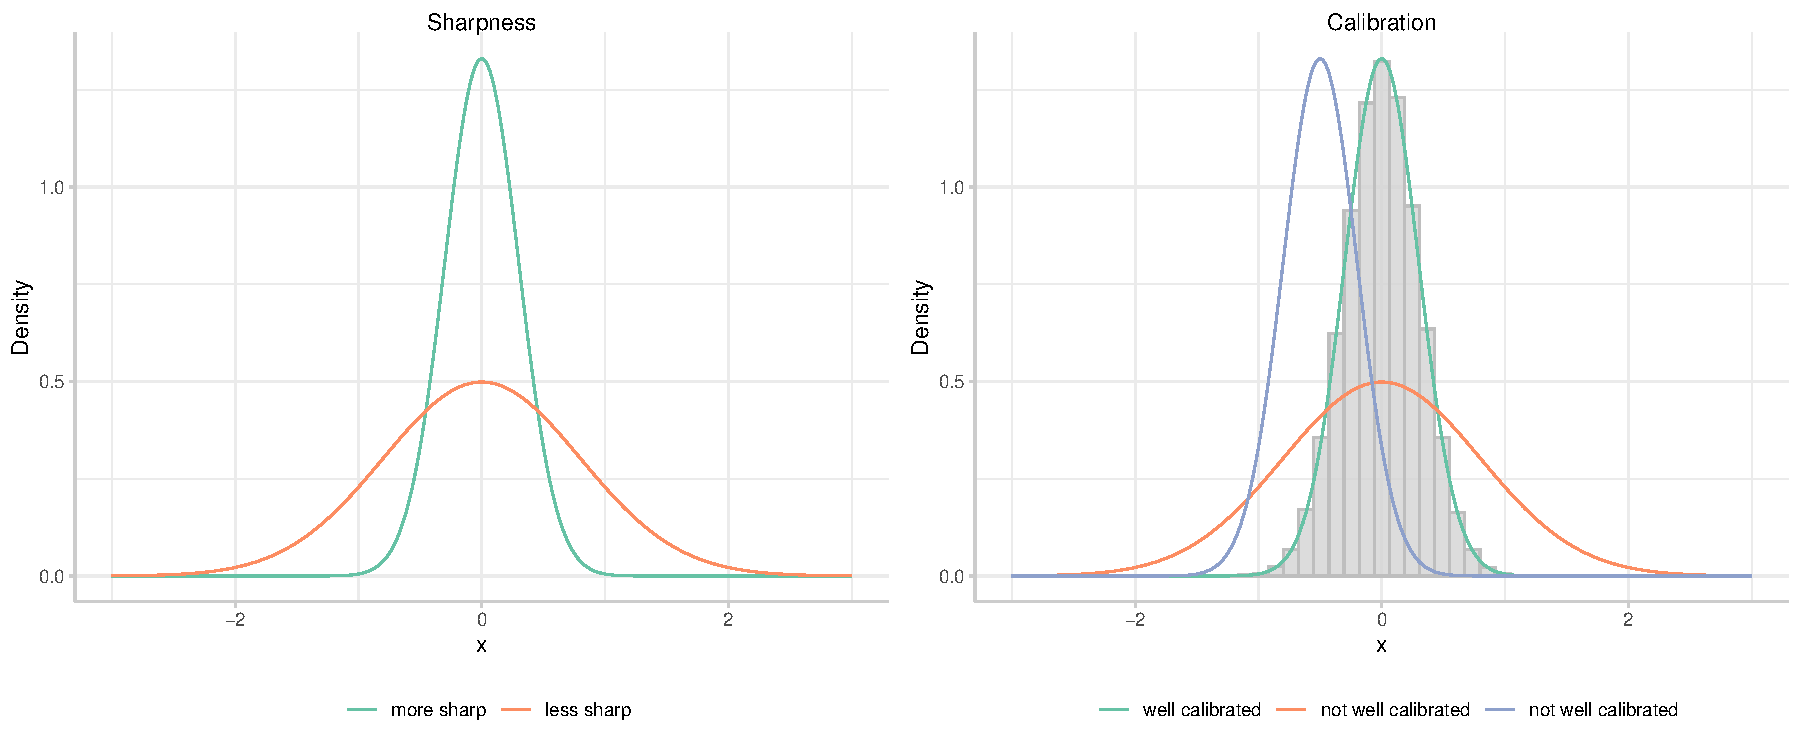
\includegraphics[width = 0.95\textwidth]{../plots/sharp_calib.pdf}
\caption{Illustration of the concepts $calibration$ and $sharpness$, as introduced by \cite{gneiting_strictly_2007}, AGAIN OTHER PAPER}
\label{fig:sharpcalib}
\end{figure}
To better understand what an optimal forecast looks like and, in the same vein, how to best assess forecast performance, we follow the established and ubiquitous paradigm defined by \cite{gneiting_probabilistic_2007}: an optimal forecasts should maximize \textit{sharpness subject to calibration}. We will now briefly explain this concept.\\
Consider that we aim to make a probabilistic forecast $F_t$ for a quantity $y_t$ at time $t$, which follows the distribution $G_t$. The ideal forecaster would thus issue 
\begin{equation}
	F_t = G_t
\end{equation}
as their probabilistic forecast. In practice, $y_t$ will eventually be observed, while $G_t$ remains an unknown and hypothetical theoretical concept. The skill of the forecaster thus needs to be judged based on the forecast-observation pairs $(F_t, y_t)$ - \cite{gneiting_probabilistic_2007} suggest to base this assessment on the concepts calibration and sharpness, which are visualized in Figure \ref{fig:sharpcalib}. \\
In their words, calibration refers to the statistical consistency between the predictive distributions $(F_t)_{t = 1,2,..}$ and the observations $(y_t)_{t = 1,2,..}$ and is comprised of several different modes - we will mention them as they become applicable, but refer to \cite{gneiting_probabilistic_2007} for a full characterization of the concept. %Perhaps the most relevant in practice, marginal calibration refers to the limits of the two distributions being equal. 
Sharpness is a feature of the predictive distribution only and simply refers to the concentration of the predictive distribution. In short, they establish the result that the notion of an ideal forecaster is equivalent to the forecaster maximizing sharpness subject to calibration. In turn, this means that calibration is not a sufficient, but a necessary condition of the forecast. When assessing forecast performance, both characteristics thus need to be judged and accounted for.\\
\subsection{Proper scoring rules}
Proper scoring rules are ideal for this task, as they incorporate this idea perfectly.\\
Now, some tools for assessing calibration. In general, calibration should be seen as a necessary rather than a sufficient condition for forecast optimality.
\subsection{PIT histograms}
\subsection{Coverage}
This is a measure of marginal calibration, that is, the limits of the two distributions being equal.
%For defining optimal forecasting and threby laying groundwork on how best to assess forecast performance, 
Then, scoring rules:\\
\subsection{Proper scoring rules}
Suppose that $y$ is the realization of a random variable under the true data-generating distribution $G$. The forecasting problem is defined by trying to issue a predictive probability distribution $F$ for the future realisation of this random variable. Further, denote $s(F,G)$ for the expectation of $\text{E}[s(F,y)]$. We then say that scoring rule $s$ is \textit{proper}, if 
\[s(G,G) \leq s(F,G).\]
Put into words, this means that the scoring rule is minimized if the true data-generating distribution is issued as the forecast distribution. Likewise, the scoring rule $s$ is \textit{strictly proper}, if 
\[s(G,G) < s(F,G).\] 
A (strictly) proper scoring rule thus incentivizes the forecaster to issue his or her true belief for the predictive probability distribution.\\
This notion of the propriety of scoring rules originated with \todos{Winkler and Murphy (1968)} and its importance in the forecasting world (hmpf) cannot be overstated - if a scoring rule for distributional forecasts is not proper, it could, for instance, incentivize a forecaster to report a more confident estimate than he or she actually believes in \todos{Thorarinsdottir 2013}. \\
Mention that aggregating across locations/... preserves propriety \citep{bracher_evaluating_2021}.\\
We also want to note here that the specific scoring rule used in an application is not a meaningless choice: as will be demonstrated in later sections, different scoring rules in practice usually induce different rankings of forecasts. In practice, the guidance is thus usually to consider several scoring rules - sometimes, a stakeholders' or decision makers might also exhibit a certain preference for forecast performance, which can guide the choice.\\
Recall the concept of sharpness subject to calibration: scoring rules assess this.
\subsection{Judging forecast performance}
We focus on evaluating model performance via two central principles, that is, accuracy (coverage/calibration) and overall predictive performance (weighted interval score). \citep{sherratt_predictive_2022}.
\subsubsection{Assessing calibration}
In general, we call a forecast that is overdispersed underconfident or conservative.
\subsubsection{PIT}
One way to assess a forecast's probabilistic calibration, that is, the congruence of the proportion of observations falling below a given threshold as observed and as they are predicted by the forecast (that is, the predictive distribution's quantiles), is through the probability integral transform (PIT) histogram \citep{dawid_present_1984}.  \\
The PIT is simply defined as the predictive cumulative distribution function's value at the observed value, that is, $p_t = F_t(y_t)$. If the forecast has good probabilistic calibration, we can expect a histogram of these transformed values to be approximately uniform. A \\
However, these can be seen as a necessary, rather than as a sufficient condition for the validity of a forecast model \cite{gneiting_probabilistic_2007}. For example, a weather forecaster that always predicts with a location's yearly stationary temperature distribution would, if also judged at yearly resolution, receive a uniformly shaped (assuming no structural shifts in the temperature's distribution\footnote{Do I hear you say climate change?}), but would be of no real use.
\subsubsection{Coverage}
Coverage assesses forecast calibration by measuring the proportion of observations that fall into the predictive distribution's respective ranges over time and comparing this to the ideally expected coverage, the $nominal$ coverage. Coverage is thus a good assessment of probabilistic calibration of forecasts.
\begin{enumerate}
\item (Empirical) Interval coverage measures the proportion of observations that fall into a central prediction interval of the distribution. For instance, for the $50\%$ prediction interval, all observations that fell within the predictive distribution's $25\%$ and $75\%$ quantiles at the respective points in time are counted and divided by the total number of observations - the goal is to be as close as possible to the nominal coverage rate of $50\%$. By assessing this for several central prediction intervals, we can additionally assess marginal calibration, that is, the congruence of the limit\footnote{We are of course only approximating by our sad finite sample ways.} distribution of the predictions with the true limit distribution as exhibited by the observed data \cite{gneiting_probabilistic_2007}. Within the literature around forecasting COVID-19, it is common to assess empirical interval coverage at the $50\%$ and $90\%$ or $95\%$ levels, to assess both the central tendency as well as the tail behavior of the predictive distributions.
\item Quantile coverage measures the proportion of observations that fall below a given quantile of the predictive distribution. It thus conveys more information than interval coverage, which does not distinguish between the upper and lower quantile of the central prediction interval. For instance, a predictive distribution could exhibit good performance at the lower tail end of the distribution, but not at the upper end, which we could thus assess. Similar to assessing PIT histograms \cite{bosse_evaluating_2022}.
\item Coverage deviation summarizes the above by averaging over the observed deviations between the empirical and nominal coverage for a set of central prediction interval. We thus obtain a parsimonious way to assess coverage across several intervals, but run the danger of losing (or even masking?) information (i.e. which interval is better).
\end{enumerate}
%%%%%%%%%%%%Then, show coverage plot of three examplary models%%%%%%%%%%%%%%%%%%
Also here, as one could just predict the historical average. At the same time, one needs a sufficiently large sample to assess coverage. Thus, a model can ``hide'' behind good coverage in the aggregate. Assessing calibration in general is thus more a necessary rather than a sufficient condition for good forecast performance. However, it is still a very useful diagnostic tool that can help forecasters assess whether they are generally over- or under-confident.\\ 
%Prediction interval coverage measures the proportion of values that fell into a predictive interval of a given level and thus reflects how well a model was able to characterize uncertainty over time.\citep{cramer_evaluation_2022} \todos{(from SI, cite something better. Scoringutils paper is also a good reference)}. It measures probabilistic calibration \citep{bosse_evaluating_2022}.
In related literature, it's common to report coverage for the central $50\%$ and $90\%$ prediction intervals \todos{(cite)}.
\subsubsection{Bias}
To assess whether a forecasting model is biased, that is, systematically over- or underpredicts the target of interest, one can utilize the bias metric as proposed by \cite{funk_assessing_nodate}. For integer-valued forecasts, they suggest the following metric:
\begin{equation*}
B(F_t, y_t) = 1 - (F_t(y_t) + F_t(y_t + 1)).
\end{equation*}
In terms of bias, the ideal forecast would have exactly half its probability mass above and below the true value $y_t$, respectively. If this is exactly the case, the metric assigns a value of zero - otherwise, if the probability mass is unequally distributed, the forecast receives a penalty. If more probability mass lies below  the true value than above it, bias is negative - the extreme case thus occurs when the entire probability mass lies below true value, where we get $B_t = -1$. The opposite applies in the case where more probability mass lies above the true value. Thus, bias measures a forecast's general tendency to relatively over- or underpredict the target \cite{bosse_evaluating_2022}.\\
\cite{bosse_evaluating_2022} extend the bias metric for quantile-based forecasts as follows. If the true value $y_t$ is below the predicted median forecast $q_{t,0.5}$, the bias is 
\begin{equation*}
B(F_t, y_t) = 1 - 2 \cdot \text{max}\{\tau | q_{t,\tau} \leq y_t \}.
\end{equation*}
Similarly, if the true value $y_t$ is above the median forecast $q_{t,0.5}$, it is
\begin{equation*}
B(F_t, y_t) = 1 - 2 \cdot \text{min}\{\tau | q_{t,\tau} \geq y_t \}.
\end{equation*}
This can be interpreted as twice the difference between the quantile level that would ideally be closest to the observed data $y_t$ ($\tau = 0.5$, since the median would be the ideal prediction) and the quantile level that is actually most in line with it. If the observed value directly coincides with the median prediction $q_{t, 0.5}$, bias is zero, otherwise, the forecast receives a penalty. Concretely, if we interpret the quantiles as the endpoints of (central) prediction intervals, this is the outermost quantile of the predictive distribution such that the interval still contains the observed value $y_t$. As above, if the entire predictive mass is above or below the observed value, bias should take on the values 1 and -1, respectively. This is achieved by simply setting $q_{t,0} = 0$ and $q_{t,1} = \infty$.\\
Thus, in short, the further the central mass of the predictive distribution is from the observed value, the larger the bias.\\
An important feature of the bias metric is that it is bound to the interval $[-1,1]$ and thereby scores forecasts on a relative rather than an absolute scale - this means that we can directly compare different targets, even if their value ranges differ substantially.
In the next subsection, we introduce the weighted interval score, which also includes penalties for over- and underprediction and can thus be used to assess a forecast's bias. However, as \citep{bosse_evaluating_2022} remark, it does so on an absolute scale - the potential issue with this is that there are no ``ideal'' absolute values for over- and underprediction and these values can thus not be directly translated into an assessment of systematic bias.
``It largely depends on the application whether one is more interested in the tendency to be biased or in the absolute value of over- and underpredictions'' \citep{bosse_evaluating_2022}.
\subsubsection{Weighted Interval Score} \label{ssub:weighted_interval_score}
Here, we introduce the \ac{wis}, which is the main scoring rule used within this thesis \cite{bracher_evaluating_2021}. It is designed for use on probabilistic forecasts \cite{european_covid-19_forecast_hub_european_2021} $F$ that are issued as a set of discrete central prediction intervals, each with nominal coverage level $\alpha$ - or, put differently, as a set of symmetric predictive quantiles $q$ which directly translate to central prediction intervals. \\
Each central prediction interval can be scored via the interval score \citep{gneiting_strictly_2007}
\begin{equation}
IS_{\alpha}(F, y) = (u-l) + \frac{2}{\alpha}(l - y)\mathbb{1}(y < l) + \frac{2}{\alpha}(y - u)\mathbb{1}(y > u),
\end{equation}
where $\mathbb{1}$ is the indicator function, returning 1 if the condition inside the parentheses is fulfilled and 0 otherwise. The three summands each have an intuitive interpretation. The second and third summands express under- and over-prediction, respectively. They assign a penalty if the true observed quantity $y$ falls below (above) the lower (upper) endpoint $l$ ($u$) of the prediction interval. The first $(u-l)$ expresses the width of the central prediction interval and thus the sharpness of the predictive distribution $F$ - if this term didn't exist, it would make sense to simply issue very large prediction intervals that are highly likely to contain the true observation $y$. These penalties are furthermore scaled by the nominal coverage level: a smaller $\alpha$, which corresponds to a higher nominal coverage rate, induces a higher penalty if $y$ does fall outside one of the endpoints. \\
\cite{bracher_evaluating_2021} extend this score for use on a predictive distribution $F$ that consists of a set of such intervals, each with unique coverage level $\alpha$. The set of interval scores is gathered and aggregated into the weighted interval score 
\begin{equation}
WIS_{\alpha_{0:K}}(F,y) = \frac{1}{K + 1/2}\left(w_{0}|y-m| + \sum_{k=1}^{K}\left(w_k IS_{\alpha_{k}}(F, y)\right)\right),
\end{equation}
where usually the quantile weights are set to $w_k = \frac{\alpha_{k}}{2}$, and the median weight to $w_{0} = \frac{1}{2}$.\\
It can be shown that the \ac{wis} is an approximation of the \ac{crps}, a well-known scoring function that measures the distance between the predictive and true distribution 
\begin{equation}
CRPS(F, x) = \int_{-\infty}^{\infty} \left(F(y) - \mathbb{1}(y \geq x) \right)^2dy.
\end{equation}
In contrast to the \ac{crps}, the WIS gives slightly larger weight to intervals with large nominal coverage \citep{bracher_evaluating_2021}.
All in all, the \ac{wis} is a parsimonious way to score forecasts that come in the shape of a set of discrete intervals \citep{sherratt_predictive_2022}. Its decomposition allows to understand it directly as summarizing the trade-off between coverage and precision. \\
An important characteristic of the WIS is that it is not standardized and thus scales with the data. This can be easily seen in equation ?, as the absolute differences of the observed value and the predicted quantile directly enter into the score. Thus, scores will naturally increase if the target to be predicted increases. This makes forecast comparisons a bit difficult, which leads us to the next point.
\subsection{Pairwise comparisons}
One issue that often arises when aiming to compare different forecasting models is a potentially non-overlapping base of targets the models predicted for, as some scoring rules are not normalized and thus scale with the data. For instance, if models were compared via average WIS, one model might look better than another if it only predicted in periods that saw low incidence or were otherwise comparatively "easy" to forecast. This would thus disincentivize forecasters to predict in periods that they perceive to be more challenging - this is especially undesirable because these periods (e.g. exponential growth, high level of infections) are often of special interest to decision makers \todos{(cite something)}.\\
One can address this by computing a relative score that is based on employing pairwise comparisons, as developed in \cite{cramer_evaluation_2022}. For a pair of models denoted $l$ and $m$, first a measure of relative skill is computed
\[
\theta_{l,m} = \frac{\bar{s}_{l}}{\bar{s}_{m}},
\]
where $\bar{s}_{l}$ and $\bar{s}_{m}$ denote the average scores the models achieved on the targets both models predicted on - this is usually chosen to be the WIS. Other scoring rules are possible, but they need to have a fixed orientiation - for instance, the log score (not further discussed here) can take on both negative and positive values, making it unsuitable for these comparisons. For each model, the geometric mean of these relative scores is then computed as
\[
\theta_{l\cdot} = \left(\prod_{m = 1}^{M}\theta_{l,m} \right)^{\frac{1}{M}},
\]to obtain a relative score of model $l$ with respect to all other available models. It can thus be interpreted as a performance measure of model $l$ with respect to a model with ``average'' performance. If interest lies in a direct pairwise comparison with a specific model $m$, one can instead consider the ratio of these relative scores
\[
\phi_{l,m} = \frac{\theta_{l\cdot}}{\theta_{m\cdot}}.
\]
Calculating this ratio for all model pairs that are of interest results in a ``pairwise tournament'' for all models in the set - this approach is implemented in the \textbf{scoringutils} package \citep{bosse_epiforecastsscoringutils_2022}. For negatively oriented scoring rules, the ratio will be smaller than 1 if model $l$ outperformed model $m$ on their set of shared targets and larger than 1 if it did not. Note that this mode of pairwise comparison still requires the assumption that it is equally hard to perform relatively well to other models at all forecast dates and locations \citep{cramer_evaluation_2022}.\\
If one is interested in concisely summarizing the skill of single models rather than performing comparisons between all pairs of models, one can choose a baseline model's $B$ relative score $\theta_{B\cdot}$ as the denominator, which for the WIS results in the measure that is commonly referred to as "relative WIS". Analogously to above, a ratio below 1 corresponds to a model overall outperforming the baseline model, while a score above 1 means that the model did not succeed in clearing baseline performance.\\
In section \ref{sub:model_types_analysis}, we use these comparisons to compare groups of models, more specifically certain model types, against each other (better: compare relative skill?). As stated previously, averaging scores preserves propriety, making this comparison possible.
\subsection{Model distance}
We so far discussed scoring rules, which, as stated, are used to assess the pairs $(F_t, y_t)$. In contrast to this, divergence functions $d$ are used to assess distance between a pair of distribution functions ($F_t$, $F'_t$) \cite{thorarinsdottir_using_2013}. This can be used to score the predictive distribution $F_t$ against an estimate of the true data generating distribution $\hat{G}_t$, but also to measure the distance between two competing predictive distributions $F_t$ and $H_t$. As it is fundamentally a measure of distance, the divergence function needs to fulfill $d(F,F)$ = 0 and $d(F,H)\geq 0$ for all $F$ and $H$. Furthermore, as they can be used to score a predictive distribution, it also needs to fulfill the notion of propriety as defined previously. Analogously to before, this means that. \\
The distance function we will use within the context of this thesis is the 2-order Cramer distance or integrated quadratic distance \cite{thorarinsdottir_using_2013}. It is defined as the integral
\begin{equation}
CD(F, H) = \int_{-\infty}^{\infty}\left(F(t) - H(t) \right)^2dt
\end{equation}
Incidentally, this is the divergence function associated with the CRPS as defined previously - this means that if a point forecast is issued instead, it reduces to the CRPS.\\
\cite{wang_covidhubutils_2022} developed an approximation of the Cramer distance for (potentially unequally-spaced) quantile-based forecasts as follows:
\begin{equation}
CD(F,H) \approx \sum_{i = 1}^{2K-1} (a_i^F - a_i^H)^2 (q_{i+1}^{P} - q_{i}^{P}),
\end{equation} 
where $q^P$ contains the $2K$ pooled and ordered predictive quantiles\footnote{With a slight abuse of notation as the subscript $i$ in this case indexes the position in the vector $q^P$, whereas usually the subscript refers to the quantile level $\tau$. However, since $\tau \in (0,1)$ and $i \in \{1,2,...,2K\}$, we believe the distinction is clear enough.} from $F$ and $H$ and $a_i^F$ is a vector that, for each quantile $q_i$ in the pooled quantile vector, contains the minimum quantile level $\tau$ for which the associated quantile $q_\tau^F$ is larger than it. We write this condition as
\begin{equation*}
a_i^F = \text{min}\{\tau | q_\tau^F \geq q_i^P\},
\end{equation*}
with an analogous definition for $H$.
Some characteristics: on the scale of the data $y_t$.\\

Explain some characteristics of the Cramer distance, i.e. that it gives small distance to distributions that are wide. Investigate this a bit.
\section{Data}
The data used in this thesis stem from the European COVID-19 Forecast Hub (thereafter referred to as the ``Hub'' or ``European Hub'', for the sake of brevity), which was instigated by the \ac{ecdc} in 2021 to collate forecasts for COVID-19 incidence cases and deaths from independent modeling teams across Europe \citep{european_covid-19_forecast_hub_european_2021}. It was modeled after a similar previous effort in the United States, the United States COVID-19 Forecast Hub (thereafter referred to as the ``US Hub'') \citep{cramer_united_2021}. Furthermore, the preceding German-Polish Forecast Hub was largely synchronized with the European Hub \citep{bracher_german_2020}. The Hub's primary goal is stated to "provide reliable information about the near-term epidemiology of the COVID-19 pandemic to the research and policy communities and the general public" \citep{sherratt_predictive_2022}.\\ 
In general, a modeling hub is a coordinated effort, in which one or more common prediction targets, as well as a common format for prediction, are agreed upon and centrally implemented \citep{reich_collaborative_2022}. This serves the purpose of facilitating model evaluation and development by making model predictions comparable, as well as making predictions suitable for aggregation, that is, for generating ensemble predictions. A central advantage of the ``Hub'' methodology is thus the potential to synthesize results from different modeling approaches and teams - for instance, \cite{metcalf_opportunities_2017} remark that, following major disease outbreaks, there is often an explosion of modeling studies, but the usefulness of the thereby generated research is limited as quality of data and methods used vary, and there is often no follow-up for synthetication of results. %, somewhat passing up the opportunity to bring the field forward. 
The Hub format, in contrast to this, standardizes data quality\footnote{To a certain degree: Teams are free to use whatever data sources they wish, but are told that forecasts will be evaluated against the publicly available JHU data and are thus recommended to base their methods on the same data source. Furthermore, the hub recommends data sources for e.g. vaccination and testing data.} and facilitates evaluation and thus synthetication of results through a set of shared targets. The format has some precedence both in other fields, for instance climatology or ecology \citep{warszawski_inter-sectoral_2014}, as well as in epidemiology itself - some notable examples include forecasting influenza in the United States \citep{reich_collaborative_2019} as well as dengue fever in Puerto Rico and Peru \citep{johansson_open_2019}. \\
\begin{figure}
\includegraphics[width = \textwidth]{plot_placeholder/visualize_data.png}
\caption{\todos{Replace with real plot.} Plot showing an example trajectory from the Czech Republic. Following the last available truth data point (on \todos{date}, modeling teams submit forecasts for one to four weeks into the future, respectively as a predictive distribution via a set of discrete quantiles. Pictured are the trajectories of the respective median predictions, with 90\% prediction intervals.}
\label{fig:czech_predictions}
\end{figure}
For these seasonal diseases, prediction targets were total number of cases in a season or the height of the peak, while in the case of the European Hub, the common prediction target are weekly incidence COVID-19 case and death counts in 32 European countries, later also hospitalization rates. Forecasts are issued in a probabilistic manner, more specifically as a set of 23 quantiles of the predictive distribution, at non-equally-spaced levels between 0.01 and 0.99. Consider Figure \ref{fig:czech_predictions} for a demonstration of the prediction format, in this case for case numbers in the Czech Republic, with the forecast date the \todos{date}. We can see that, ...\\ 
There were no restrictions for participation in the Hub, (meaning that in theory anyone could participate) and participating teams or individuals were free to only submit forecasts for any subset of combinations of locations and target types. Forecast dates were standardized and based on the \ac{ew} format as defined by the US \ac{cdc}, where each week starts on a Sunday and ends on the following Saturday. Forecasts were submitted by Monday and thus scored against the truth data as realized on the Saturday of the same week for 1-week ahead forecasts, and accordingly by the following Saturdays for larger horizons.\\ 
The truth data source that models are evaluated against stem from the \ac{jhu}, which collate and make available daily cumulative counts of cases and deaths. Since the Hub asks for weekly forecasts of incidence, the truth data is obtained by taking weekly differences of the \ac{jhu} national data. This can in theory be problematic, as data are subject to revision and negative values for incidence counts are thus possible.\\
To be included in the official Hub's ensemble, models had to provide a full set of 23 quantiles for all four forecast horizons, as well as pass a sequence of automated checks for their predictions, that is, that their quantile predictions were non-negative, integer-valued and did not cross \citep{sherratt_european_2022}.\\
\begin{figure}
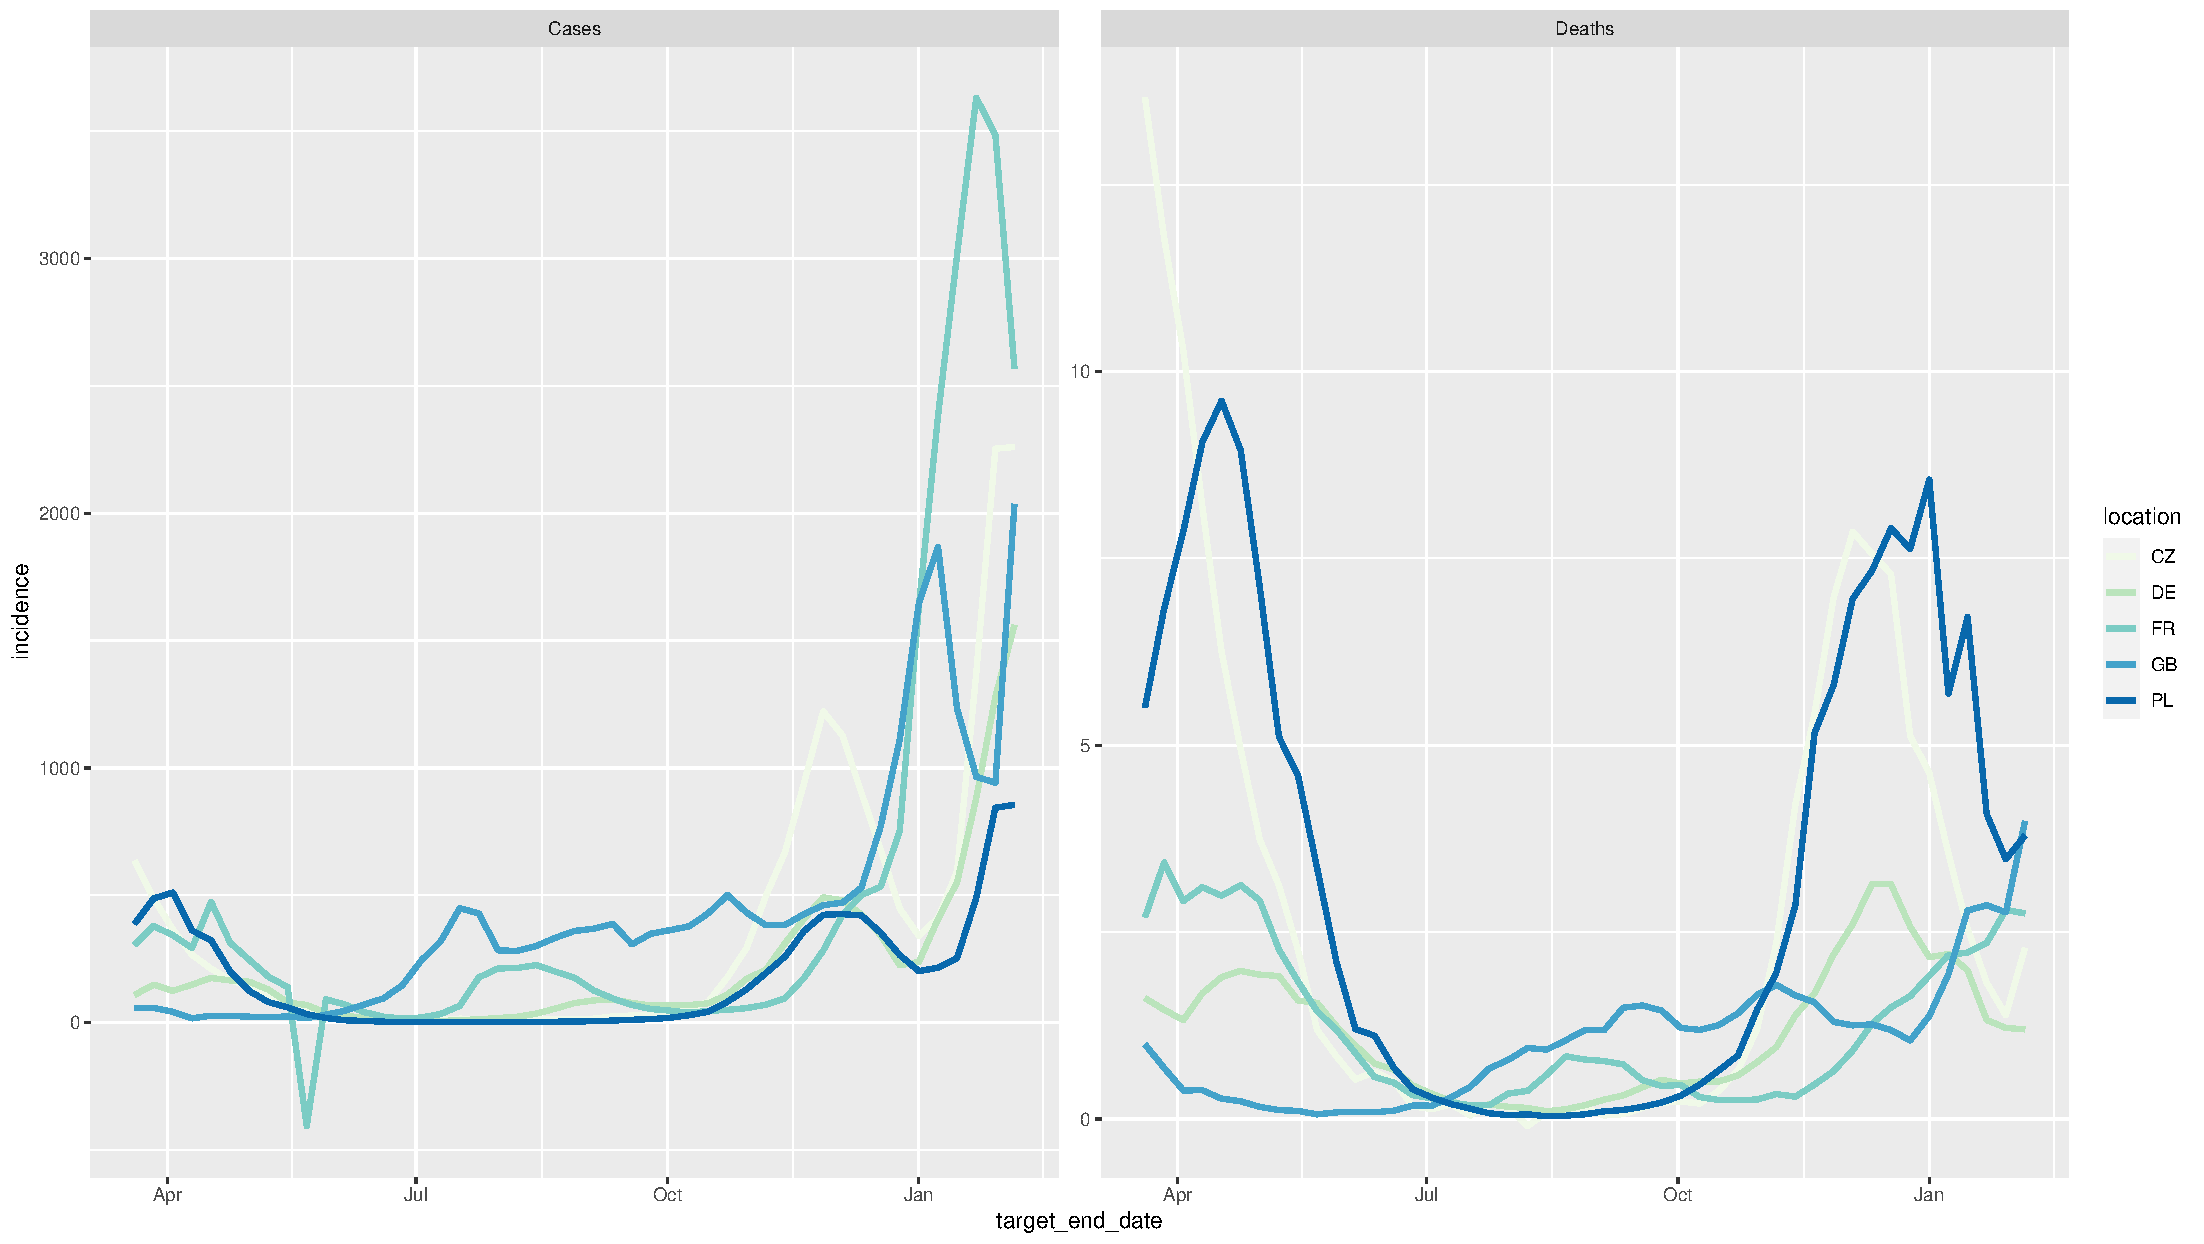
\includegraphics[width = \textwidth]{../plots/trajectories.pdf}
\caption{Plot showing the trajectories of the different time series. Note that the time series for Cases were normalized by the respective location's population for readability. Time series for deaths are direct incidence counts.}
\label{fig:trajectories}
\end{figure}
\begin{figure}
\includegraphics[width = \textwidth]{../plots/availability_indivi.pdf}
\caption{Plot showing the overall availability of each model submitted to the European COVID-19 Forecast Hub across the five locations considered in this study. It can be seen that there is large variability in the availability of each model. Some models are available during most of the study period, while others only submit forecasts for a small section of the considered period. It can also be seen that there are some models that submit predictions for several or most locations, while others only predict for one specific location.}
\end{figure}
The Hub also includes a ``naive'' baseline model, which is the same as the one that is used in the US Covid-19 Forecast Hub \cite{cramer_evaluation_2022}. For each forecast date, its forecast for median incidence is equal to the last value for incidence Cases/Deaths that was observed in the most recent week. For uncertainty around the median, the other predictive quantiles are taken from Monte Carlo approximations of the empirical distribution function that is induced by the first differences observed in the respective time series \citep{cramer_evaluation_2022}. In essence, this model can thus be seen as a martingale/random walk model with non-stationary variance. On the one hand, including a baseline model serves the purpose of providing a sort of ``minimum'' performance that models should be able to clear - reporting that a model performs better than the baseline thus gives validity to the performance of that model. On the other hand, given the fact that most prominent scoring rules scale with the target and thus never obtain a sort of ``optimum'', it's a pragmatic strategy to compare performance across dimensions that are usually not easily comparable, for instance across different periods or locations. Furthermore, adding a relative model that serves as a sort of measure of forecasting difficulty rather than relying on absolute performance also serves as a sort of dis-discouragement of inviting teams to forecast during periods that are perceived as more ``difficult'' than others (and which additionally also receive nominally very high scores). However, we want to note here that while the introduction of a baseline aims to fulfill the purpose of standardizing model comparison, it is not without alternative and can skew the assessment somewhat if it systematically performs better in some dates than others: as we will see, there are some periods which the baseline fails at. As \cite{bracher_evaluating_2021} ``showed''(?), the choice of baseline can impact model assessment and is not entirely trivial.\\
For both the European and US Hub, the central communication tools lies with the Hub ensemble, which was generally found to perform best. In both cases, it was found that the median  \\
Talk about how the ``ensemble is best'' paradigm has also held here, with citations to both Eu and Us FCH.\\
Talk about issues of model availability.\\
\subsection{Hub Data}
\begin{figure}
\includegraphics[width = \textwidth]{../plots/availability_indivi.pdf}
\caption{Plot showing the overall availability models submitted to the European COVID-19 Forecast Hub across the five locations considered in this study.}
\end{figure}
For the subset used in this study, we decided ahead of our study to only use a subset of the available countries in the set. This is simply due to the fact that most of the analyses we aimed to perform required a sufficient model base as support. Furthermore, we decided to only use data up until the end of January of 2022. This is due to the fact that model base dropped around Christmas,. Moreover, beginning with the new year 2022, Omicron\textsuperscript{TM} entered the chat and in some countries, testing criteria changed. We thought that this could make the time periods less comparable.\\
Talk about availability. We can see that in the aggregate, after an initial period of uptake and recruiting, the modeling base is largest during the summer months and into the fall of 2021, after which it drops.
In general, the varying model base can be a bit of an issue. One can deal with these issues by e.g. only taking a full forecast set. However, we deliberately wanted to deal with the data as-is and develop and conceive strategies that work with and around this artefact of the data, as we felt that this was the most realistic and helpful for the situation at hand. \\
We restricted ourselves to models that submitted the full set of 23 quantiles for each of the four horizons.\\
Formally, we can thus write that each forecast $i$ at time $t$ is issued as a set of 23 quantiles for horizons $h$ between 1 to 4 weeks ahead: $q_{i, t, h, \tau}$, where $\tau \in \{0.01, 0.025, 0.05, 0.1, ... 0.9, 0.95, 0.975, 0.99\} $. Note that quantile levels are not equally spaced, giving the predictive distributions a higher resolution around their respective tails. These quantile levels directly induce 11 central prediction intervals with nominal coverage level $(1-\alpha)\%$, with $\alpha \in \{0.02, 0.05, 0.1, 0.2, ... 0.9\}$.\\
For the US forecast hub, some things have worked well, most notably best performers or weighting. The question is whether we can also come to similar conclusions here. Especially for Death forecasts, best performers seemed to work well in the US forecast hub (see: https://covid19forecasthub.org/doc/ensemble/).
%%%%%%%%%%%%%%%%%%%%%%%%%%%%%%%%%%%%%%%%%%%%%%%%%%%%%%%%%%%%%%%%%%%%%%%%%%%%%%%%%%%%%%%%%%%%%%%%%%
%%%%%%%%%%%%%%%%%%%%%%%%%%%%%%%%%%%%%%%%%%%%%%%%%%%%%%%%%%%%%%%%%%%%%%%%%%%%%%%%%%%%%%%%%%%%%%%%%%
%%%%%%%%%%%%%%%%%%%%%%%%%%%%%%%%%%%%%%%%%%%%%%%%%%%%%%%%%%%%%%%%%%%%%%%%%%%%%%%%%%%%%%%%%%%%%%%%%%
%%%%%%%%%%%%%%%%%%%%%%%%%%%%%%%%%%%%%%%%%%%%%%%%%%%%%%%%%%%%%%%%%%%%%%%%%%%%%%%%%%%%%%%%%%%%%%%%%%
%%%%%%%%%%%%%%%%%%%%%%%%%%%%%%%%%%%%%%%%%%%%%%%%%%%%%%%%%%%%%%%%%%%%%%%%%%%%%%%%%%%%%%%%%%%%%%%%%%
%%%%%%%%%%%%%%%%%%%%%%%%%%%%%%%%%%%%%%%%%%%%%%%%%%%%%%%%%%%%%%%%%%%%%%%%%%%%%%%%%%%%%%%%%%%%%%%%%%
%%%%%%%%%%%%%%%%%%%%%%%%%%%%%%%%%%%%%%%%%%%%%%%%%%%%%%%%%%%%%%%%%%%%%%%%%%%%%%%%%%%%%%%%%%%%%%%%%%
%%%%%%%%%%%%%%%%%%%%%%%%%%%%%%%%%%%%%%%%%%%%%%%%%%%%%%%%%%%%%%%%%%%%%%%%%%%%%%%%%%%%%%%%%%%%%%%%%%
%%%%%%%%%%%%%%%%%%%%%%%%%%%%%%%%%%%%%%%%%%%%%%%%%%%%%%%%%%%%%%%%%%%%%%%%%%%%%%%%%%%%%%%%%%%%%%%%%%
\section{Introspective stuff}
This section, as well as the next, will largely be devoid of rigorous statistical testing. Most of the works cited in this thesis that perform evaluations of similarly are. There exist methods to test the significance of differences in forecast scores/skill between models, the most common being the Diebold-Mariano test, which however has no extension ``to account for dependencies between multiple forecasts made for different time series or locations''(\cite{bracher_evaluating_2021}, \cite{diebold_comparing_1995}). One could also conceive a regression analysis, e.g. with random effects, but this also has the issue that scores are correlated and scores have large outliers which can heavily influence and thus weaken the trust in reported p-values. We still think there is tremendous value in the analysis, but we are aware of and want to highlight the possible limitations. We argue that some of the knowledge distilled in this thesis should be checked against another year's results, to increase trust in the results. Furthmore, \cite{bosse_epiforecastsscoringutils_2022} don't recommend statistical testing ``in applied settings''.\\ 
We try to counteract this by carefully not masking trends in the aggregate, as well as also reporting results that did not show any striking conclusions. Most of our analysis leads were furthermore defined from the start, and we refrained from \todos{(take this out, as it's not entirely true?)}.\\
\subsection{Model Types} \label{sub:model_types_analysis}
First and foremost, we had to categorize the models in the data in a meaningful manner. We decided on a categorization. To this end, we . Teams that mentioned an explicit compartmental structure of SIR or related (for instance SEIR, SECIR) type we categorized as "mechanistic".\\
As stated before, the question of which modeling strategy or type is the best choice for short-term infectious disease forecasting remains an ongoing topic of research \cite{funk_short-term_nodate}. For the case of influenza, \cite{reich_collaborative_2019} found that statistical models exhibited similar or better performance than compartmental models in short-term forecasts of ``influenza numbers'' (except for 1-wk ahead) and \cite{the_influenza_forecasting_working_group_collaborative_2019} similarly found that statistical models outperformed mechanistic models, thereby suggesting that mechanistic assumptions (and thus explicitly modeling the epidemiological process) need not necessarily improve short-term predictive performance \cite{funk_short-term_nodate}.\footnote{generally, the performance differences were greater for larger horizons, include this?}. In the case of the latter study, statistical models - interestingly - performed best in relation to mechanistic ones in a period that saw a highly atypical pattern, `` illustrating that the statistical approaches may be more resilient to predictable patterns in ILI''.\\
However, as discussed previously, results from one disease don't necessarily transfer to another, especially when they show fundamentally differing characteristics, that is, seasonal vs. emerging. In the case of COVID-19, \citep{bracher_evaluating_2021} state that they did not find any ``striking patterns'' between model types in their analysis, but also acknowledge that this might be due to the relatively short study period they considered (12 weeks). A question that thus naturally arises is, whether given a longer study period, patterns can be found.\\
\begin{figure}
\centering
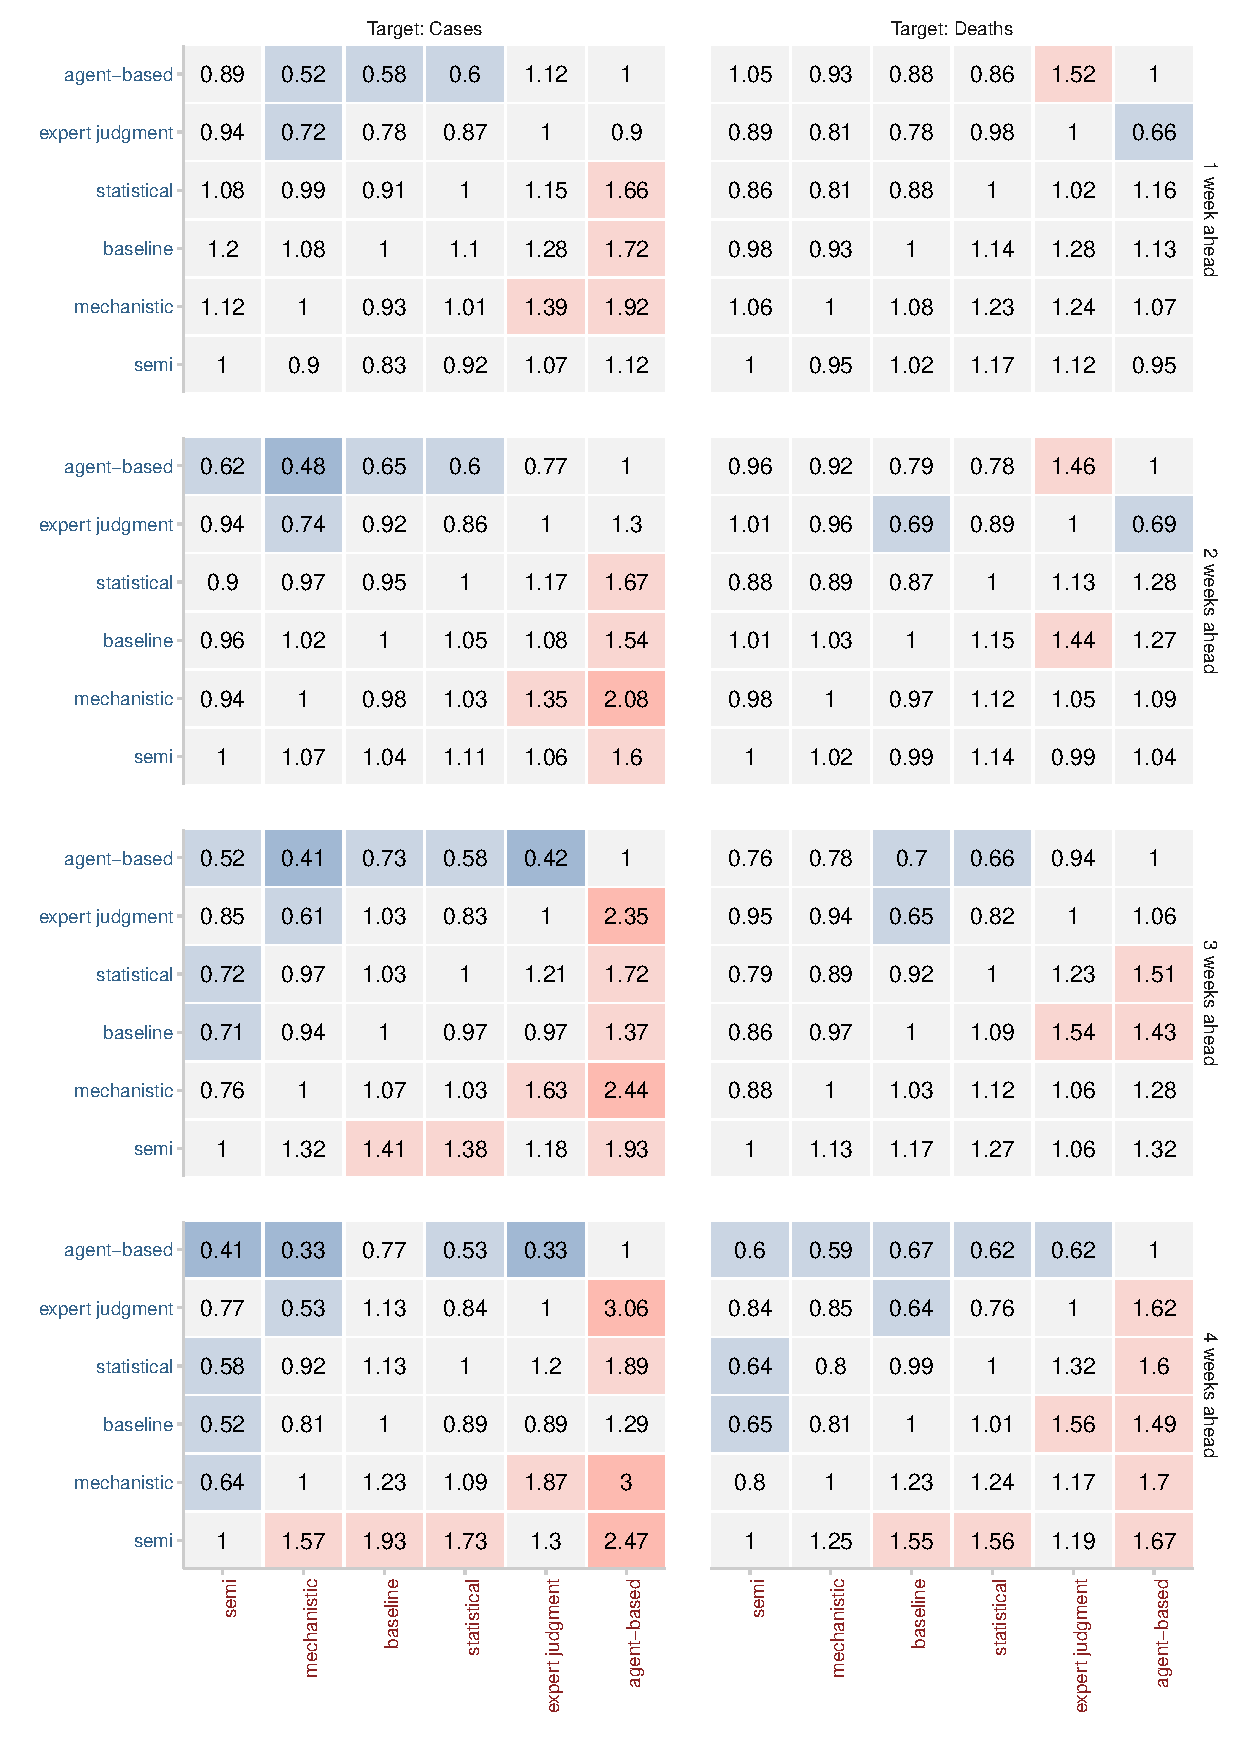
\includegraphics[width = 0.9\textwidth]{../plots/pw_comp_model_type_with_other.pdf}
\caption{Pairwise comparison of model types. Plot was produced with package \texttt{scoringutils}}
\label{fig:pw_comp_modeltypes}
\end{figure}
%%%%%%%%%%%%%%%%%%%%%%%%%%%%%%%%%%%%%%%%%General intro to evaluation method/data base%%%%%%%%%%%%%%%%%%%%%%%%%%%%%%%%%%%
Typically, the recommendation is to only compare models which are available for at least $50\% $ of the time period under study, to avoid comparison of forecasts that don't have any overlap \citep{bosse_epiforecastsscoringutils_2022}. Since we are however comparing forecasts at the level of model types rather than single models and there does not exist a pair of model types without overlap in the relevant time period, this advice does not necessarily apply here. One could still make the argument that one should not exclude models that only contribute for a very small portion of the study period, so as not to have models that more likely produce outlying forecasts\footnote{One could think that models that only have e.g. $10\%$ availability either dropped out due to not performing well and/or teams might have not been invested enough in the project to update and keep tuning their model, both of which might give low-quality predictions that as a result might not necessarily be representative of the respective model type.} influence the results too much - however, we found that the results were not at all sensitive to the exact choice of availability threshold chosen for the models, so we decided not to exclude any models here.\footnote{results from exclusions can be found in appendix} \\ 
Nevertheless, there remains the issue of the more obscure model types: as previously stated, the two agent-based models in the set only submitted forecasts for Poland, while the expert-judgment based models dropped out of the Hub during the late summer period of 2021. We report their results the highest level of aggregation (averaged results across all locations and forecast dates), but will mostly leave them out in the subsequent analyses, for conciseness and as we think that dwelling on their performance too much might give non-generalizable results. Note that the value of the mean score ratio between two model types in the pairwise comparisons is independent of other models in the set, so the mean score ratios of the other pairs are unaffected by this choice \todos{WRONGGGGGG}.\\
%%%%%%%%%%%%%%%%%%%%%%%%%%%%%%%%%%%%%%%%%%%%Discuss pairwise comparisons%%%%%%%%%%%%%%%%%%%%%%%%%%%%%%%%%%%%%%%
The results of the pairwise comparison, where for each model type, weighted interval scores are stratified by horizon and target type, but averaged across the entire study period and all locations, can be found in Figure \ref{fig:pw_comp_modeltypes}. These plots show that the only modeling strategy that tends to show consistent increased performance improvement over other model types are agent-based models. It seems that, compared to other model types, they perform particularly well for forecasting case numbers, even more so at longer horizons. As previously mentioned, within our data set, these models only issue forecasts for Poland (for both Cases and Deaths), so the comparisons are purely based on the data from that location. Thus, it is unclear whether their superior performance would transfer to other locations or settings. In particular, most other models (and thus model types) in the data set make forecasts for multiple locations, and one could argue that designing and tuning a model for a specific location lacks some of the potential complications that arise when aiming to establish a model with more universal application. We thus argue that comparability is very limited.\\
Apart from this, we see some substantial differences in skill between expert judgment forecasts and mechanistic models for case forecasts. Upon investigation, \todos{(investigate where this comes from)} \\
We argue that perhaps the most interesting observation can be seen at horizons three and four: we see that semi-mechanistic models are outperformed by both mechanistic and statistical models for longer horizons. This could be due to the case that models based on growth rate are more vulnerable to overprediction at longer horizons, as (slight) overprediction of the growth rate, through the multiplicative nature of the underlying epidemiological process, can lead to larger overpredictions of the target. \\
  %are , so they don't necessarily receive the same level of care and effort. As previosuly sta \\
\begin{figure}
\centering
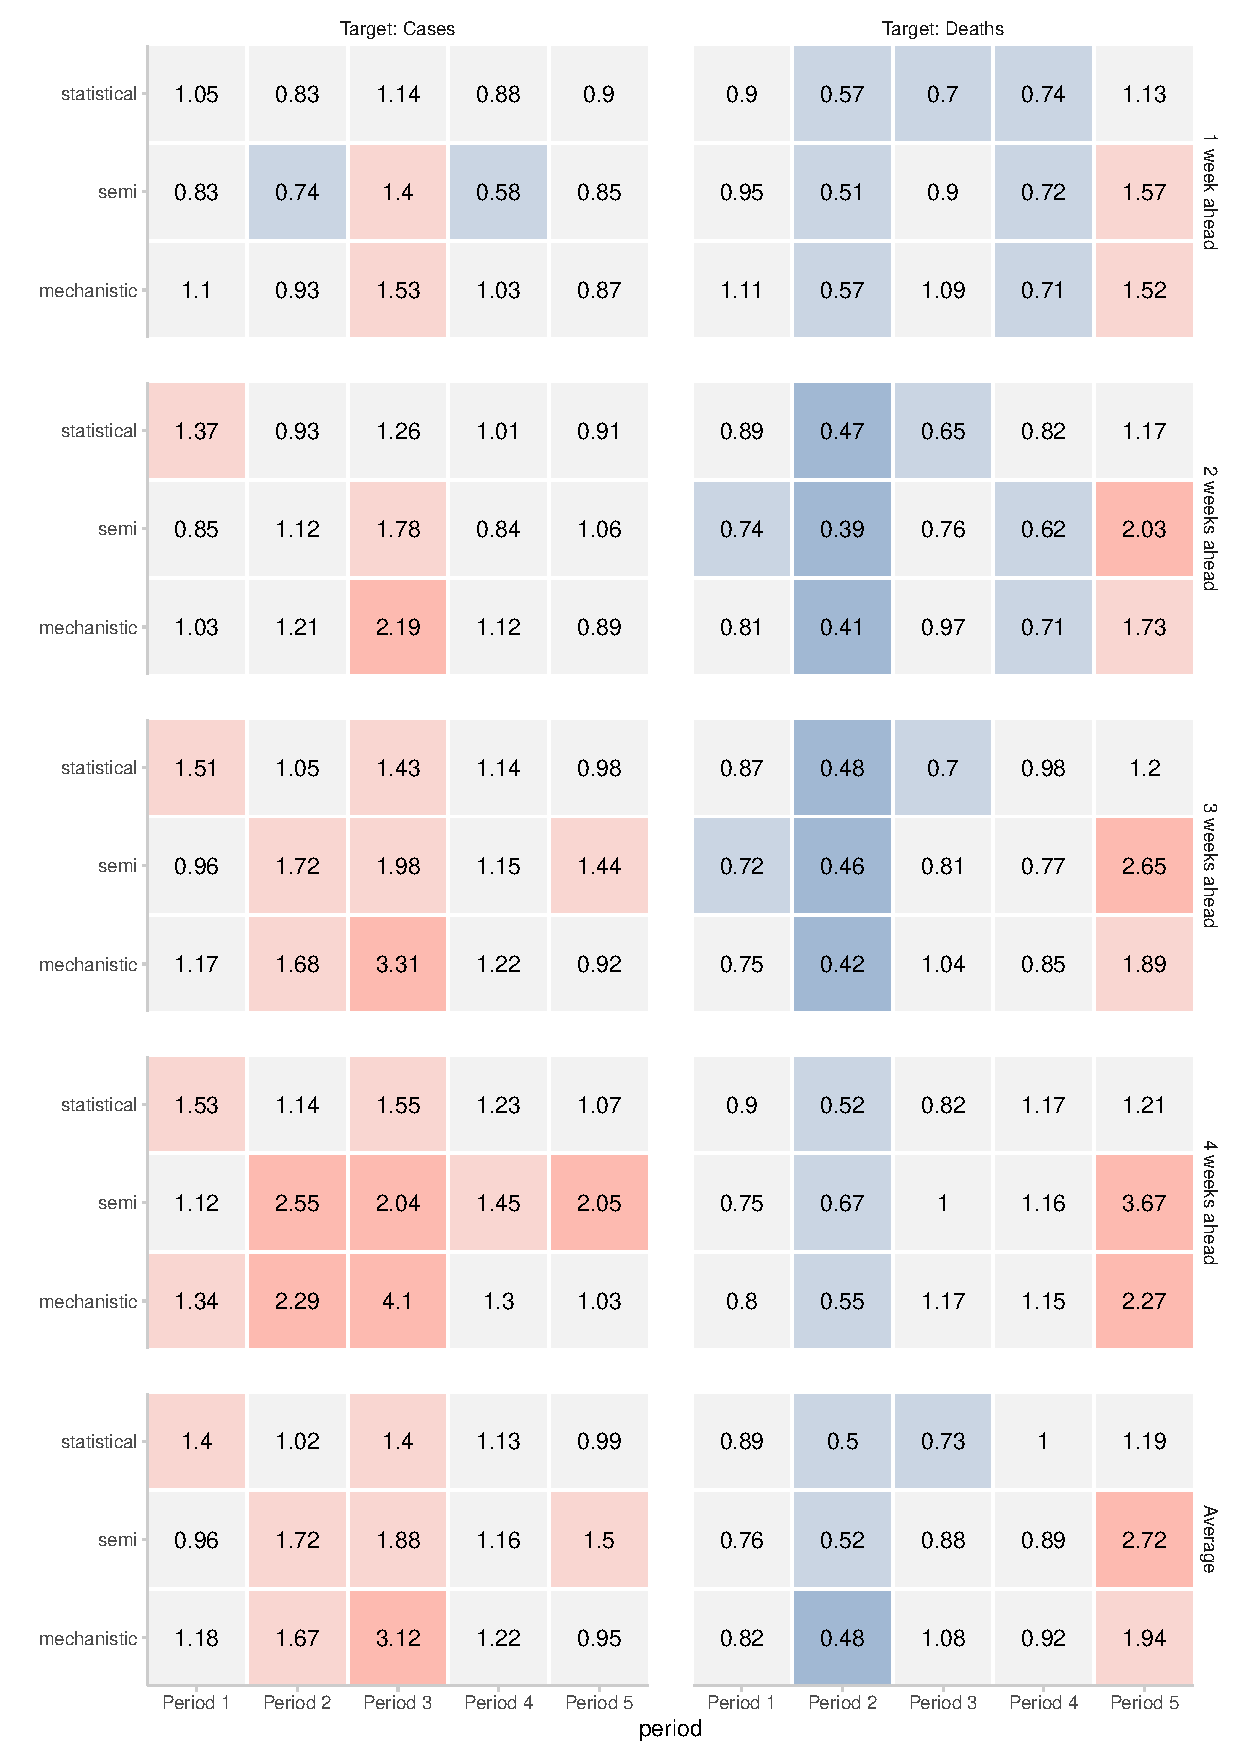
\includegraphics[width = 0.7\textwidth]{../plots/pw_comp_model_types_across_periods.pdf}
\caption{Pairwise comparison of chosen model types across time periods. The code to produce this plot was adapted from package \texttt{scoringutils}}
\label{fig:pw_comp_modeltypes_byperiod}
\end{figure}
Of course, averaging across the entire study period and all locations has the issue of potentially masking some trends or effects, or worse, presenting trends in the aggregate that perhaps only spuriously result from diverging results at a lower resolution. Furthermore, as previously stated, average WIS scores are generally vulnerable to domination by periods and locations with high nominal incidence levels, thus making it possible that these results only stem from e.g. locations with larger populations.\\ 
First of all, we thus want to evaluate whether the results presented above describe a consistent trend across the entire time period, or whether these only stem from certain phases of the trajectories. We thereby follow \cite{taylor_combining_2021} in dividing our study period into 10-week periods\footnote{since we have 47 weeks in our studied sample, we actually divide into 2 10-week and 3 9-week periods}, to investigate whether these trends hold. The results can be found in Figure \ref{fig:pw_comp_modeltypes_byperiod} For conciseness, we refrain from showing all pairwise comparisons and only report performance against the baseline.\footnote{However, as can easily be seen from equation XX, if a model type has a lower mean score ratio with respect to the baseline model than another model type, it will also outperform that model type in terms of the mean score ratio.}
First of all, we can see that performance is heavily correlated across model types, that is, we observe more variations between the periods overall than between the model types. Hence, we can say that there are some periods which are harder to predict in comparison to the baseline, while during other periods this is easier. %Recall that models here are scored against a baseline model which predicts median levels to be the same in the future: this model is harder to beat in period 3, where Cases .
%%%%%%% Across horizons and locations
- we see that bad semi scores mostly seem to derive from period 5. while e.g. mechanistic models also underperform in some periods, these periods do not influence the aggregate too much.
- scores are correlated\\
- Statistical models better in period 5, for both deaths and cases. This is in line with Bracherboy \todos{(actually, not really)}.\\
Recall what we previously stated about some periods being easier to forecast in comparison to the baseline: this is especially obvious in period 2, where death numbers are mostly marked by decline and low levels overall (see Figure \ref{fig:trajectories}), we observe that all model types markedly outperform the baseline model at virtually all horizons and locations. Investigating the decomposition of baseline WIS during this period, we found that the baseline model's dispersion alone sat between 0.96 (at horizon 1) and 1.46 (at horizon 2) of the \textit{overall} average WIS score of all other model types, suggesting that the baseline model issued severely underconfident forecasts during this time. \footnote{Does this mean that the baseline model was badly calibrated? Also, find out if this was especially the case during the beginning of a period. Argument could be: baseline not so well adapted to falling numbers, where other models manage to be more confident.} Since the baseline model's uncertainty bands are based on past differences, this suggests that these don't update quick enough, marking the point that the choice of baseline is not entirely trivial. \\
\todos{(consider again the next section, might be wrong. How does averaging work again? ... See scoringutils paper.)}
To see that scores are relatively heavily dominated by periods and locations with high nominal incidence, consider the results from case forecasts in period 3 in Figures \ref{fig:pw_comp_modeltypes_byperiod} and \ref{fig:pw_comp_modeltypes_byloc}: all model types substantially underperform with respect to the baseline in the aggregate, but they actually outperform the baseline for Poland and the Czech Republic. Since these countries however have very low incidence numbers compared with other countries in the evaluation set during this period (see Figure \ref{fig:trajectories}), they don't influence the average score very much. Whether or not this is a desirable feature of the evaluation method is an ongoing debate and can depend on the forecasters' as well as decision makers' preferences. For instance, \cite{bracher_evaluating_2021} argue that scoring forecasts in this manner is meaningful, as a fixed relative deviation from the observed quantity can be regarded as more problematic at high incidence levels rather than at very low incidence levels, which would not be accounted for if only considering the relative deviation.\\  
%%%%%%%%%%%%%%%%%%%%%%%%%%%%%%%%%%%%%%%%%%%%%%Discuss decomposition%%%%%%%%%%%%%%%%%%%%%%%%%%%%%%%%%%%%%%%%%%
As explained in subsection \ref{ssub:weighted_interval_score}, the weighted interval score can straightforwardly be decomposed into penalties accrued from overprediction, underprediction and dispersion. A question that thus naturally arises is whether the score differences discussed previously can be explained by model types performing particularly well or not with respect to a certain component. To this end, we show the decomposed average WIS scores obtained by each model type in Figure \ref{fig:decomp_model_types}. Note that these are the raw average scores rather than scores obtained relative to the baseline model. This is possible since forecasts from all model types are available for the entire time period under study and we first averaged by forecast date and then by model type\footnote{arggh, not actually true. Statistical models missing for the first few weeks in CZ, FR, GB. Could put figure in appendix showing robustness}. We hence see that scores vary substantially more between the different forecast horizons than they do between the model types, but that we can nevertheless observe some interesting facts. 
- Lastly, we also see a general result from previous studies: cases get increasingly harder to forecast than deaths at higher forecast horizons.\\
- For both targets, forecasts from semi-mechanistic models receive higher penalties for overdispersion than the other model types.\\
- For both targets, forecasts from statistical models receive higher penalties for underprediction than the other model types.\\
- relatively bad performance for semi-mechanistic models at longer horizons (while higher overdispersion throughtout, semi-mechanistic models additionally accrue high scores for overprediction at longer forecast horizons.)\\
- for death forecasts, mechanistic models have higher overprediction component\\
- one could of course argue that 4-week ahead predictions are relatively unreliable anyway \\
Interestingly, statistical models more commonly receive penalties for underprediction. It's interesting here to mention that through the multiplicative nature of the underlying epidemiological process, it is often "safer" to score models in terms of underprediction than overprediction in terms of absolute WIS scores.\footnote{We want to pull attention to forthcoming work by Nikos Bosse, who investigates scoring forecasts in terms of relative rather than absolute errors.}  \todos{(remove this, as the thought is definitely inspired by Nikos' paper and I can't cite it?)}\\
Furthermore, Figure \ref{fig:decomp_model_types} shows that semi-mechanistic models tend to be better calibrated, that is, show closer to nominal coverage rates than other model types - this is especially true at the $90\%$ level for both targets, and at the $50\%$ level for case forecasts, while these models are slighty underconfident for death forecasts at the $50\%$ level, where the group of statistical models is almost perfectly calibrated. This shows a common trade-off: as shown by the decomposition of the WIS, semi-mechanistic models lack sharpness, but this seems to allow them better calibration, while other model groups issue sharper forecasts at the expense of not containing as many of the observations as they are meant to. As stated in \cite{sherratt_european_2022}, the Hub ensemble suffers from increased overconfidence for Cases with rising forecast horizon on top of general sub-nominal coverage levels, which suggests that these models still might enter favorably into the ensemble by helping to counteract that overconfidence. Whether this actually holds true, we will investigate further in section XX. Generally, we however see a trend of overconfidence for all model types for both targets and furthermore we see a bit of a downward trend in the coverage ratio with rising horizon, especially for case forecasts - this is in line with the results for models in \cite{sherratt_european_2022}. \\
This is again likely due to the case that ``this group on average'' overpredicts in large absolute terms, particularly in period 5, but in general seems to be somewhat well calibrated (?)...\\
Of course, all of this comes with a caveat. Not really a consistent pattern.
\begin{figure}
\centering
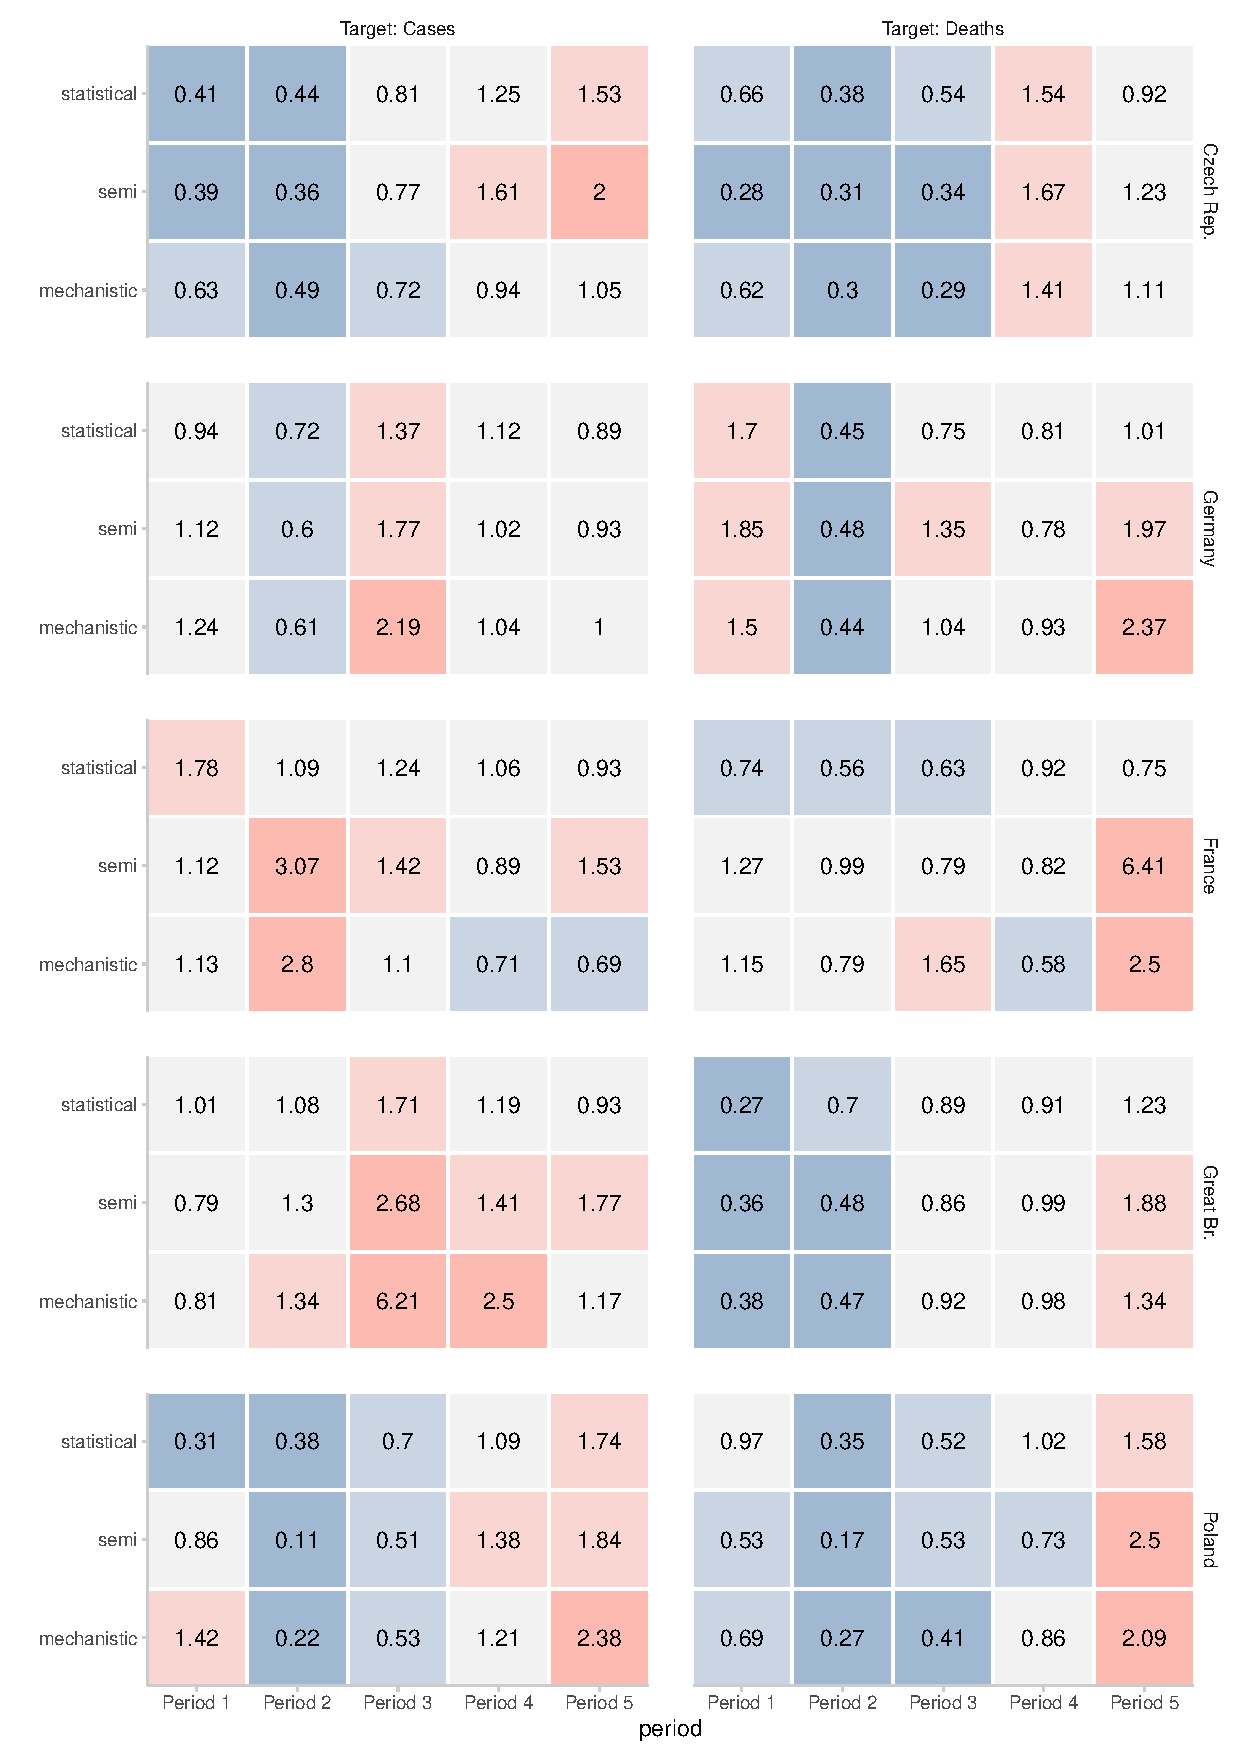
\includegraphics[width = 0.9\textwidth]{../plots/pw_comp_model_types_across_periods_and_loc.pdf}
\caption{Pairwise comparison of chosen model types across locations. The code to produce this plot was adapted from package \texttt{scoringutils}}
\label{fig:pw_comp_modeltypes_byloc}
\end{figure}
\begin{figure}
\centering
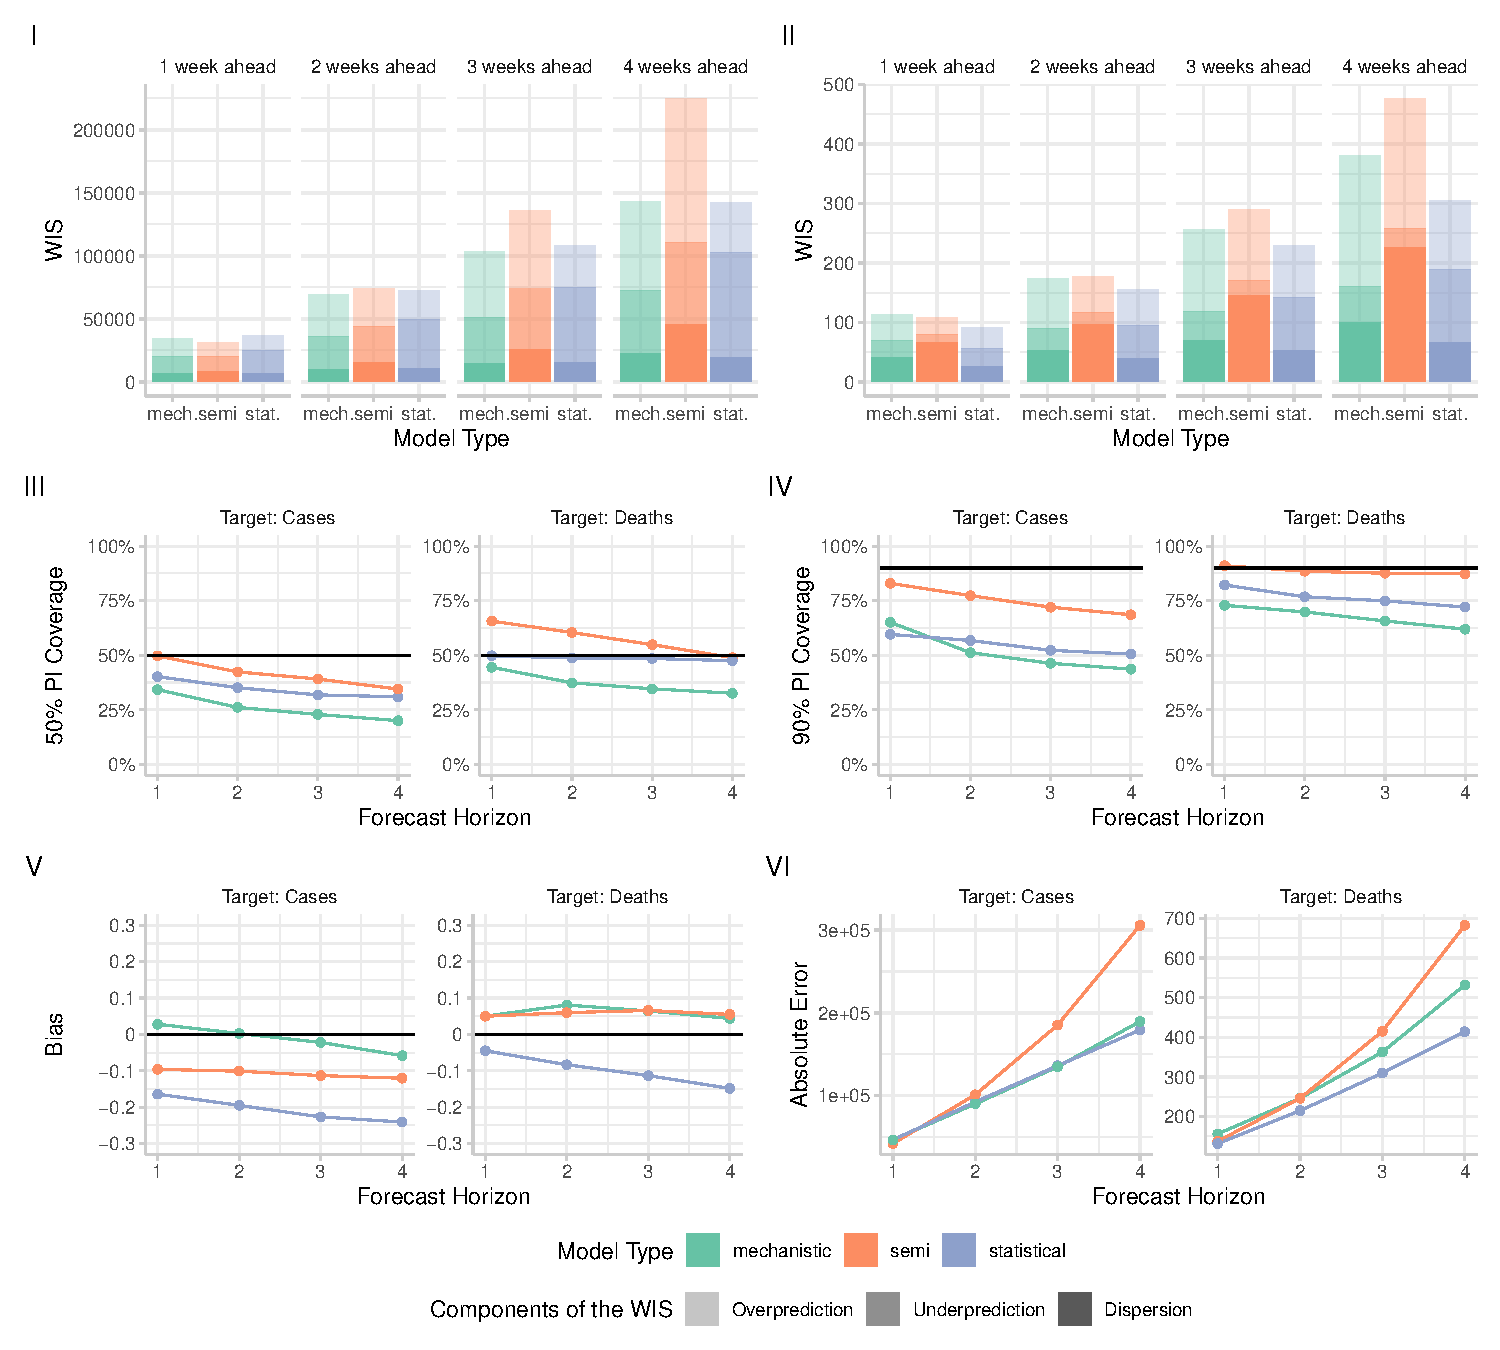
\includegraphics[width = 0.95\textwidth]{../plots/overall_assessment_model_types.pdf}
\caption{Figure showing performance with respect to several scoring rules of the three dominant model types (mechanistic, semi-mechanistic, statistical) in the European Forecast Hub, across five locations over the time period March 2021 - January 2022, for two targets (case and death forecasts) and forecast horizons one to four weeks into the future. Respectively, the depicted scoring rules are: (I), (II) Decomposition of the weighted interval score into overprediction, underprediction, dispersion. (III) Empirical coverage of the $50\%$ prediction interval. (IV) Empirical coverage of the $90\%$ prediction interval. (V) Forecast bias, which ranges between -1 and 1. (VI) absolute error of the median forecasts. Wherever applicable, the desired target value of the score is shown as a black solid line - for all other scoring rules, a lower value of the score corresponds to better performance. Plot heavily inspired by \cite{bosse_comparing_2021-1}. \todos{replace line plots with box plots}}
\label{fig:decomp_model_types}
\end{figure}
\subsection{Model Similarity}
We now turn to the issue of model similarity in ensembles. As expanded upon in Section \todos{XX}, ensemble models are widely regarded to be successful due to the fact that they counteract/mitigate individual model biases and furthermore reduce variance by aggregating a number of models. Regarding the first point of mitigating bias, it is thus conceivable that ensembling approaches could be less successful if some of the included models are too similar. To illustrate this, recall the , thereby skewing 
%include plot of scaled model similarity
%plot of model performance with respect to number of models kicked out
%analyze which models are actually similar 
This notion has some mention (\todos{find better word}) in the literature. For example, in \cite{bosse_comparing_2021-1}, the authors mention that they purposefully did not submit one of their models for inclusion in the forecast hub's ensemble, as there was concern that it could be too similar to another model they already submitted. However, this decision based on the two models' similarity in modeling setup (shortly explain), rather than on an actual judgment of how close their predictions were. Nevertheless, they did find that both models improved the ensemble if included \todos{(find out if this was actually true)}. We now want to do a more systematic review of this concept - since we will consider more models across more countries, we hope to get a more accurate picture.\\
\begin{figure}
\centering
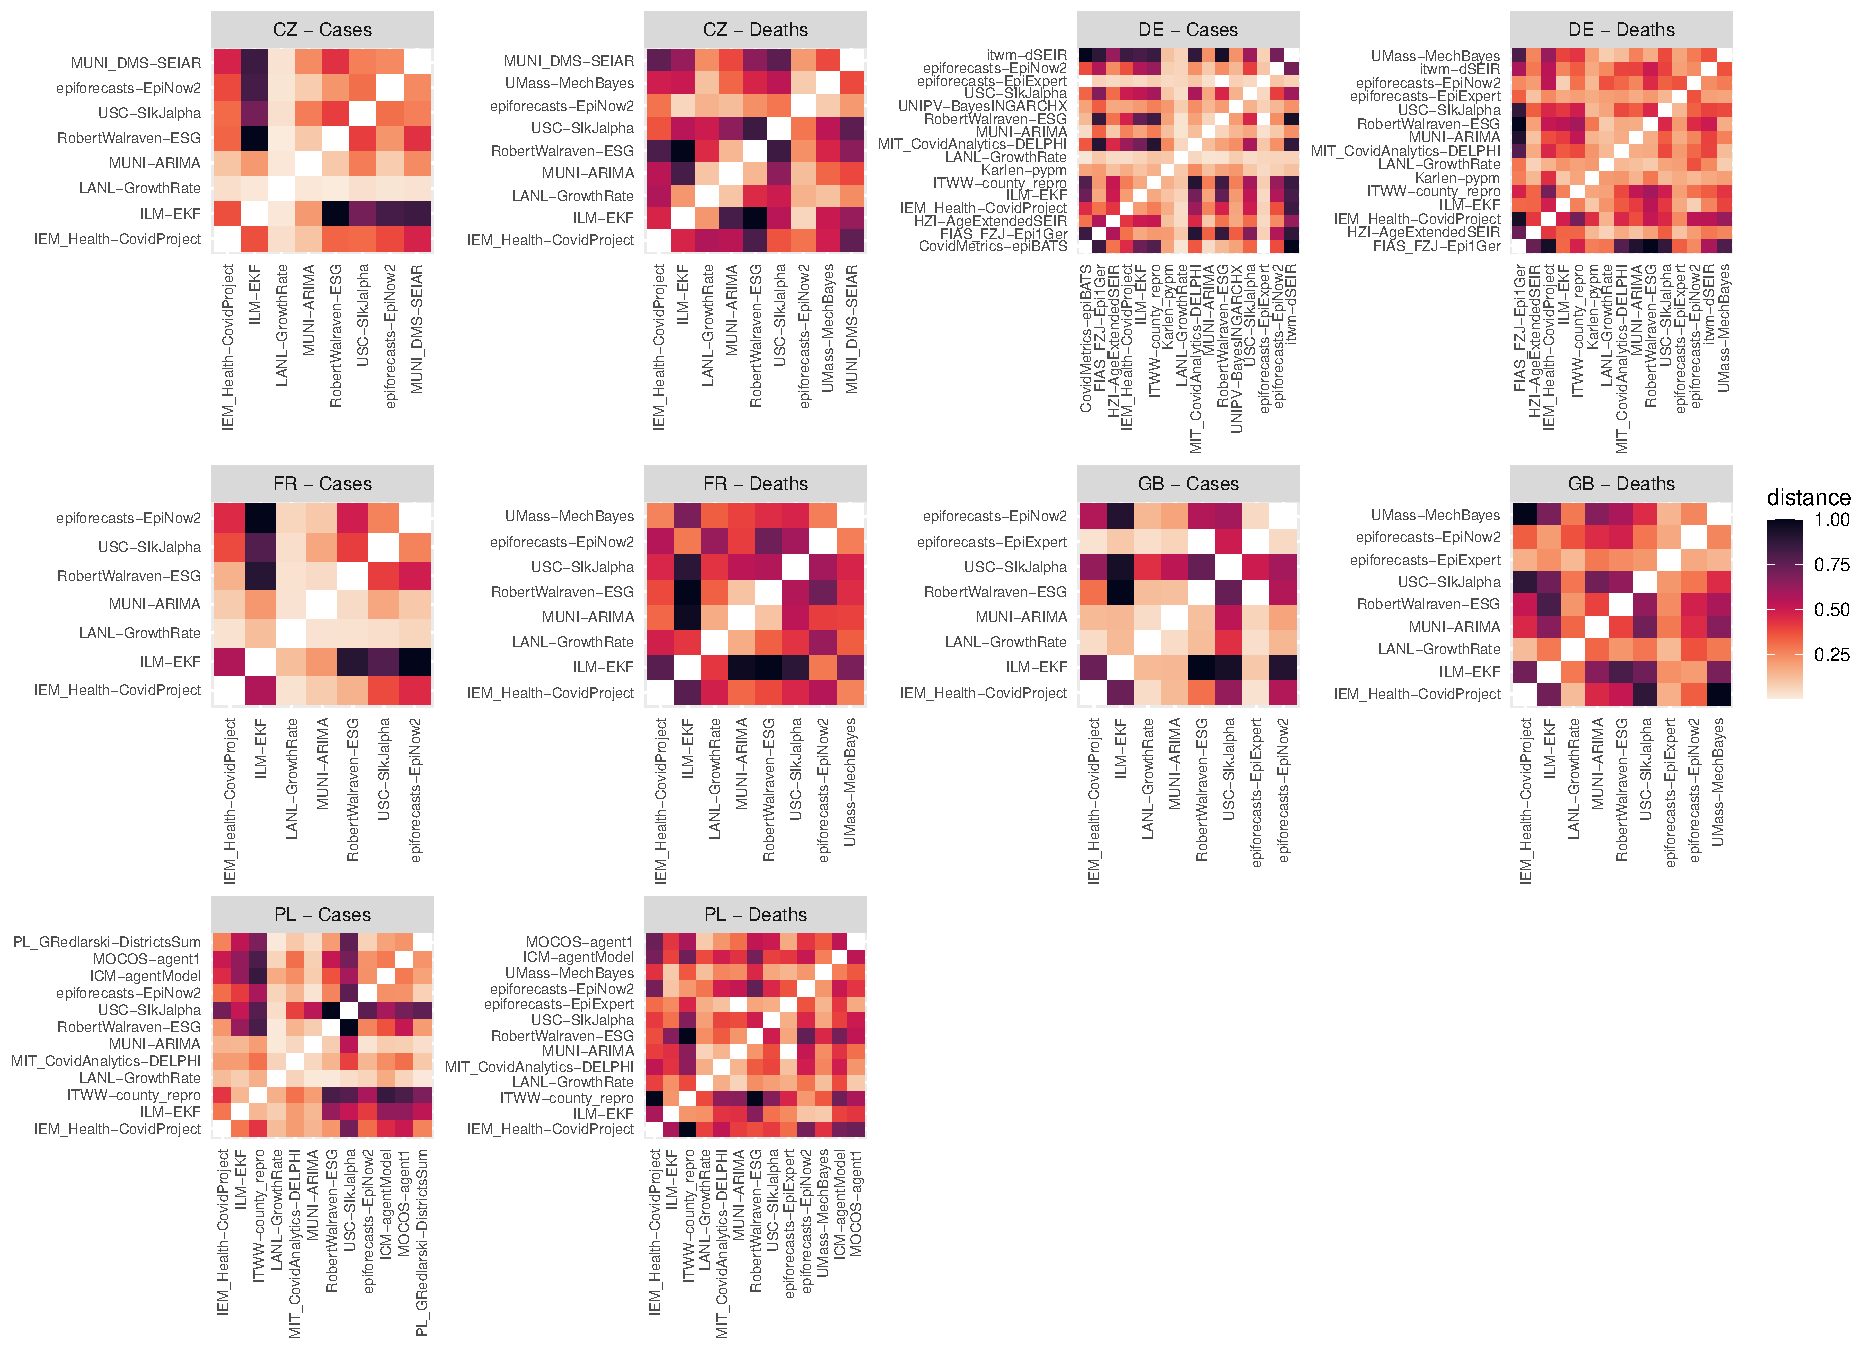
\includegraphics[width = 0.95\textwidth]{../plots/model_similarity.pdf}
\end{figure}
\newpage
\subsection{Ensemble Techniques}
- Mean, median \\
- weighted, different types of weight computes: QRA, inverse score weighting, inverse score weighting with exponential smoothing.
Weighting by past performance: the most natural choice as a score is again the weighted interval score, as it is the most parsimonious way to score forecasts in terms of both calibration and sharpness. 
\subsection{Adding a new model}
``To enhance
interpretability of scores we mainly report WIS relative to the Hub ensemble in the main text, i.e. we divided
the average scores for a given model by the average score achieved by the Hub ensemble on the same set of
forecasts (with values >1 implying worse and values <1 implying better performance than the Hub ensemble).''\cite{bosse_comparing_2021-1}.
We thus designed the following experiment: for each forecast date, we first built every possible ensemble of size $n$ from the available models at that date. The problem with investigating ensemble size as it relates to performance in the dataset is that, as amply mentioned beforehand, the actual realized ensemble size is not constant as models drop in and out of the Hub, while we also have no universal measure of absolute forecast skill, and one would need to disentangle ensemble size from the inherent level of difficulty present at a given forecast date. In a regression, one could of course control for these idiosyncrasies, but as also mentioned beforehand, scores are not suited as the dependent outcome in a regression and we are furthermore left with the problem of not having a lot of data. But, if we have data on the average score of an ensemble of size $n$, we can study the (expected) added benefit of adding another model to the ensemble. This has some interesting dimensions that we want to explore:\\
- are there times (high vs. low incidence is what most easily comes to mind) where adding a model is more beneficial?\\
- is adding a model more beneficial for the mean or the median ensemble? \cite{bosse_comparing_2021-1} found that performance changes from adding or removing a model from the ensemble were ``of a similar order of magnitude, suggesting that at least in this instance, with a relatively small ensemble size, the median ensemble was not necessarily more ``robust'' to changes than the mean ensemble''. They find also that adding a 
- are there differences between adding a model that is more vs less distant to the current ensemble?
- how much does individual model performance matter? How "safe" is it to add any model, even if it might be a bad performer? We deliberately chose the ``perfect knowledge situation'' where we knew about actual current model performance. 
- are there models that if added provide a particularly good benefit?\\
We see that adding a very close model has almost no impact on the mean ensemble, while it does move the median ensemble. Since the median is a more discrete measure, its predictions are more skewed by adding another model. \\
Of course, this has the downside of limiting the maximum ensemble size that can be studied. This can better enhance understanding of ensemble behavior. To our knowledge, such an experiment is novel in the literature. 
%%%%%%%%%%%%%%%%%%%%%%%%%%%%%%%%%%%%%%%%%%%%%%%%%%%%%%%%%%%%%%%%%%%%%%%%%%%%%%%%%%%%%%%%%%%%%%%%%%
%%%%%%%%%%%%%%%%%%%%%%%%%%%%%%%%%%%%%%%%%%%%%%%%%%%%%%%%%%%%%%%%%%%%%%%%%%%%%%%%%%%%%%%%%%%%%%%%%%
%%%%%%%%%%%%%%%%%%%%%%%%%%%%%%%%%%%%%%%%%%%%%%%%%%%%%%%%%%%%%%%%%%%%%%%%%%%%%%%%%%%%%%%%%%%%%%%%%%
%%%%%%%%%%%%%%%%%%%%%%%%%%%%%%%%%%%%%%%%%%%%%%%%%%%%%%%%%%%%%%%%%%%%%%%%%%%%%%%%%%%%%%%%%%%%%%%%%%e
%%%%%%%%%%%%%%%%%%%%%%%%%%%%%%%%%%%%%%%%%%%%%%%%%%%%%%%%%%%%%%%%%%%%%%%%%%%%%%%%%%%%%%%%%%%%%%%%%%
%%%%%%%%%%%%%%%%%%%%%%%%%%%%%%%%%%%%%%%%%%%%%%%%%%%%%%%%%%%%%%%%%%%%%%%%%%%%%%%%%%%%%%%%%%%%%%%%%%
%%%%%%%%%%%%%%%%%%%%%%%%%%%%%%%%%%%%%%%%%%%%%%%%%%%%%%%%%%%%%%%%%%%%%%%%%%%%%%%%%%%%%%%%%%%%%%%%%%
%%%%%%%%%%%%%%%%%%%%%%%%%%%%%%%%%%%%%%%%%%%%%%%%%%%%%%%%%%%%%%%%%%%%%%%%%%%%%%%%%%%%%%%%%%%%%%%%%%
\section{Ensemble Experiments}
Some of these techniques came up . We thus retroactively analyze other ensembling methods. In light of the fact that . One could in theory denote a holdout set, but given the fast changes in disease characteristics, the periods are not really comparable.\\ 
While this is a retroactive analysis, it is generally important that it, to the extent that it is possible, simulates the real-time. That is, only information that is available up to that point in time may be used for building the ensemble. This is because we want to trial (and if successful, suggest) methods that in theory could be deployed in real-time. Otherwise, it would be too easy to retroactively devise strategies that outperform the ensemble.\\
Generally, for all "ensemble experiments", the sets of models that would enter the ensemble were automatically stratified by target type, location and of course the forecast date. Theoretically, one could also stratify by horizon.\footnote{Or even quantile? As done by US hub in ensemble experiments.} The reasoning for this is clear: some models or model types might be better at forecasting certain horizons than others. However, this could lead to things going entirely haywire \\
Note that we refrained from excessively tuning hyperparameters in the study.
We wanted to derive methods that accounted for the fact that weight estimation does not work well in low signal-to-noise ratio settings \cite{claeskens_forecast_2016}.\\
We decided to implement an ensemble that is based on the results from 1, i.e. that namely excludes semi-mechanistic models at longer horizons. Of course, we also saw that mechanistic models had rather poor performance at longer horizons, but we decided to exclude only semi-mechanistic as we otherwise wouldn't have much of an ensemble left at all. Furthermore, while the trend isn't $100\%$ clear, we mostly see that semi-mechanistic models perform either second-worst or worst. Also, while we identified a general tendency for larger dispersion (which might actually aid the generally overconfident ensemble), we additionally at larger horizons saw a much more problematic tendency to overpredict the target. We will do this analysis for both cases and deaths, but of course expect larger benefits for case forecasts. Compared with both the relative scores of the other model types, we see that semi-mechanistic models are rarely a good performer when compared to the other model types.  We of course expect this to improve performance in-sample, but further we want to investigate whether this introduces any unwanted effects, i.e. discontinuities. Namely, there are a few desirable properties of forecasts that could be in jeopardy if the set of models in the ensemble varies with the forecast horizon. It is thus conceivable that these models increase the cone of uncertainty for lower horizons, making it drop afterwards if they are then excluded. Furthermore, we also monitor the resultant coverage of the ensemble before and after, to see if anything worsened in this regard - wis might drop (not a surprise, as this is how it was selected), but that makes monitoring other scoring rules even more important. \\
For evaluation, we use a more direct relative WIS, since there are no missing forecasts in this part of the analysis.\\
Our analyses in the previous chapters showed some (if slight) performance differences of 
\subsection{Model Types}
These compartmental models, via a set of differential equations, explicitly model how members of the population transition through the states of being susceptible, (exposed), infected, and recovered/removed \cite{taylor_combining_2021}.
\cite{taylor_combining_2021} conjecture that during periods of low incidence, mechanistic models should perform better than statistical ones. This is due to the fact that random statistical fluctuations can still occur, but statistical models might, somehow, latch on to these too eagerly and proceed to forecast exponential growth where there is none.\\
Weighting at the level of model types also has the advantage of being able to use all models, even if they newly enter into the hub.\\
Two problems with inverse score weighting that shrinkage towards equal weights can fix: \\
- can overweights on e.g. statistical (which could be problematic because past predictive power is of course not a perfect; overshoot after exponential growth)
- we don't optimize for performance at all. Linear combination of two weights is of course not super flexible, but it gives at least a small dial for actual performanc eoptimization to happen. 
\subsection{Best performers}
The rationale behind this approach is that it is to a certain degree less flexible than choosing true weights, i.e. a sort of shrinkage method.\\
For this approach, we scored models based on their performance in the past four weeks. To assess this performance, we only scored forecasts that had resolved by the current forecast date, in order to better mimic the real-time situation. This means that we excluded forecasts if they were made before the current date, but for a horizon that as yet lay in the future relative to the current date. The set of scored targets thus included one 4-week ahead forecast, two 3-week ahead forecasts, three 2-week ahead forecasts and four 1-week ahead forecasts.\\
For , we also excluded those forecasts that did not realize yet, i.e. forecast date + horizon > current date.
Furthermore, in the US context, there was some success in only limiting the best performers to contribute to the ensemble.\\
Notice that here the procedure is different to what we did in section XX: we are actively removing models from the set, while in section XX we investigated the effect of adding a model to the ensemble.\\
Discuss why it might have worked well in the US, but not here.
\subsection{Weighting based on model types}
As stated before, weighting might not be the best idea. However, in practice there might be correlations of forecast performance - in sofar as this happens at the level of model types, one might be able to exploit that.\\
It is perhaps overeager to assume that one model type could systematically outperform another over the entire study period which, after all, comprises different countries with varying periods of infection dynamics. One could however then conjecture that in specific situations, one modeling philosophy could be better suited than another. For instance, \cite{taylor_combining_2021} have surmised whether in periods of low infection rates, [ensembles of] compartmental models might be best suited for forecasting, while \citep{bracher_pre-registered_2021} have identified that following changes in trends, statistical models perform more poorly, likely because they first have to observe the changing trend in the data from which they extrapolate.\\
To echo this, during our investigation of model types in section ??, we also observed that , although these did not necessarily follow any strict rules as outlined above. Nevertheless, if we for instance regard Figure ??, we can most prominently see for e.g. France that model type performance varies by period, with one type dominating the other at certain times. It would thus have been preferable to use only one type of model. Thus, we want to investigate whether these relative performance differences can be picked up by an automatic weighting scheme. \\
Schreib irgendwas darüber warum vielleicht ein Modelltyp einem anderen theoretisch überlegen sein könnte in bestimmten Phasen. Statistical exponential,... This might be hard to implement explicitly, but automatic weighting might work.\\
We aimed at categorizing phases of the pandemic into some notion of (``stable'', ``upswing'', ``downswing''), but ultimately found that any such categorization would be arbitrary to a non-neglectable degree. And anyway, results from previous section did not show robust trends. Instead, the idea is to use recent performance of the model types to weight them differently in an ensemble. As mentioned, due to models dropping in and out of predicting, there are substantial gaps for each model and thus not yielding a consistent record of recent performance that one could use to weight on. On the level of model types, we don't have these gaps. The idea thus is to first build an ensemble for each model type in the data and then to weight these respective ensembles with respect to their recent performance. The hope is that if there are periods of the pandemic where a certain model type has an edge over others, this system will recognize this and weight the models accordingly. \\
The strategy was as follows: we first built a median ensemble based on each group of model types. We chose the median ensemble as it is more resistant to outliers, which can be more problematic in the smaller group of models that were created here.\\
We decided to use an exponential weighting scheme to assess the recent score of model types. We felt that such a weighting scheme would strike a good balance between bias and variance when estimating recent performance of a model: using only a few recent observations to build average performance gives low bias, but also increases variance due to possible random fluctuations in model performance. Exponential weighting of the scoring history gives more weight to recent scores, but also includes faraway scores to a lesser degree so as to reduce the variance of the estimation.\\
\todos{(maybe include weighting as in recent Brooks/Ray/Reich paper?)}
\subsection{Overall}
Is mean or median better in period 5? Would expect median to be more robust in times of stark growth.
\section{Contributions}
A lot of work has been done on the US forecast hub. We wanted to investigate whether improvement gains could be made in a setting with a smaller model base and less consistent submissions. Sherratt showed that weighting did not work.
\begin{figure}
\centering
\includegraphics[width = 0.95\textwidth]{plot_placeholder/perform_ensemble_ovrtime.png}
\caption{From \cite{ray_ensemble_2020}. Plot different ensemble techniques over time}
\
\end{figure}
\begin{figure}
\centering
\includegraphics[width = 0.95\textwidth]{plot_placeholder/perform_ensemble_ovrtime2.png}
\caption{From \cite{ray_ensemble_2020}. Plot different ensemble techniques over time}
\
\end{figure}
\bibliography{references}
\bibliographystyle{plainnat}
\end{document}